\chapter{Marco teórico}
\label{ch:2}

En este capítulo se ofrecerá un resumen del estado del arte en el ámbito del aprendizaje por refuerzo y aprendizaje profundo por refuerzo, dando a conocer las nociones básicas de los métodos que los comprenden, así como sus aplicaciones en el control eficiente de dispositivos HVAC.

\section{Aprendizaje por refuerzo}

El \textbf{aprendizaje por refuerzo} es un método de aprendizaje computacional centrado en la interacción de un agente con su entorno. Se trata de un aprendizaje iterativo, basado en prueba y error, donde el agente recibe recompensas positivas si sus acciones le conducen a estados deseables. El objetivo del agente será, por tanto, descubrir qué acciones le conducen a la maximización de dicha recompensa \cite{sutton2018reinforcement}.

Este modelo de aprendizaje está inspirado en la psicología conductista y el condicionamiento clásico, tratando de modelar el aprendizaje animal desde la perspectiva computacional del aprendizaje automático. Clásicamente, el campo del aprendizaje automático ha sido mayoritariamente definido como la unión de los paradigmas del \textit{aprendizaje supervisado} y \textit{no supervisado}. No obstante, si los comparamos con el \textit{aprendizaje por refuerzo}, encontramos aspectos significativos que permiten diferenciarlos:

\begin{itemize}
    \item En comparación con el \textbf{aprendizaje supervisado}, basado en el aprendizaje a partir de ejemplos previamente etiquetados por un supervisor externo, en el ámbito del \textit{aprendizaje por refuerzo} el agente debe ser capaz de aprender a partir de su propia experiencia. Esto hace que el \textit{aprendizaje supervisado} pierda valor en problemas donde el aprendizaje se produce en base a la interacción.
    \item Por otro lado, también existen diferencias con respecto al \textbf{aprendizaje no supervisado}, centrado en el descubrimiento de patrones en conjuntos de datos no etiquetados. Aunque tanto el \textit{aprendizaje no supervisado} como el \textit{aprendizaje por refuerzo} carecen de ejemplos de comportamiento ``correcto'', el \textit{aprendizaje por refuerzo} trata de maximizar una señal de recompensa, en lugar de intentar encontrar patrones ocultos en los datos.
\end{itemize}

Ante esta diferenciación, podemos considerar el \textit{aprendizaje por refuerzo} como un paradigma adicional dentro del aprendizaje automático.

\subsection{Conceptos básicos}

Tal y como se muestra en la Figura \ref{fig:rl-model}, un problema de \textit{aprendizaje por refuerzo} (en adelante, RL) queda definido por los siguientes componentes:

\begin{itemize}
    \item Un \textbf{agente} que aprende a partir de la interacción con su entorno y que persigue un determinado objetivo. Las interacciones entre el agente y el entorno se producen en una serie de \textbf{pasos} o \textit{timesteps}. En cada paso, el agente observa el \textit{entorno}, realiza una \textit{acción} y recibe una nueva \textit{observación} y \textit{recompensa}. Un \textbf{episodio} es una secuencia de \textit{pasos}, que parte de un \textbf{estado inicial} y termina en un \textbf{estado terminal}\footnote{En caso de encontrarnos ante un \textit{problema continuado}, como es el caso del problema tratado en este trabajo, no existe un estado terminal como tal. En estas situaciones es necesario establecer una limitación temporal o máximo número de \textit{pasos} que determine la finalización de los episodios.}.
    \item Un \textbf{entorno}, definido como todo elemento externo al agente. Se trata de un proceso dinámico que produce datos relevantes para el agente.
    \item Un conjunto de \textbf{estados} u \textbf{observaciones} que representan la situación actual del \textit{agente} en el \textit{entorno}. Dependiendo de si la percepción del \textit{entorno} por parte del agente es total o parcial, hablaremos de \textit{estados} u \textit{observaciones}, respectivamente. El espacio de estados puede ser finito o infinito, donde cada estado queda definido por un conjunto finito de variables.
    \item Una serie de \textbf{acciones} que determinan las dinámicas del \textit{entorno}. El \textit{agente} realiza \textit{acciones} sobre el \textit{entorno} que le permiten transitar entre diferentes \textit{estados}.
    \item Una función de \textbf{recompensa}. Se trata de un valor numérico que valora cómo de ``buena'' es una \textit{acción} o \textit{estado} para el \textit{agente}, por lo que puede corresponderse con una señal positiva (estado/acción deseable) o negativa (estado/acción a evitar). Uno de los principales retos del RL es conocer las consecuencias a largo plazo de las decisiones tomadas, cuya recompensa podría demorarse en el tiempo.
    \item Una \textbf{política} que determina, para cada \textit{estado}, la probabilidad de ejecutar cada una de las \textit{acciones disponibles}. Determina el comportamiento del agente y su preferencia ante diferentes estados o acciones.
\end{itemize}

\begin{figure}
    \centering
    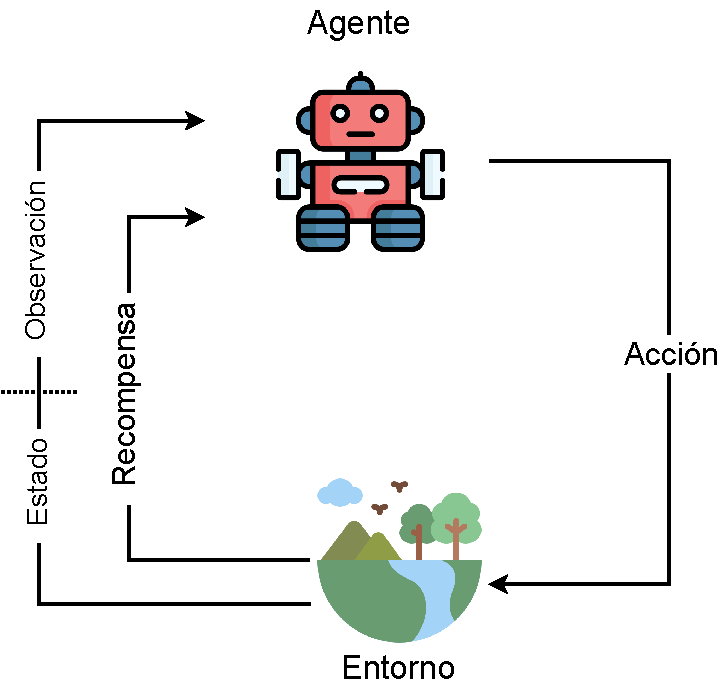
\includegraphics[width=0.6\textwidth]{imagenes/rl-components.pdf}
    \caption{Interacción \textit{agente}-\textit{entorno} en RL}
    \label{fig:rl-model}
\end{figure}

A diferencia de otros tipos de aprendizaje, a la hora de abordar un problema desde la perspectiva del RL es necesario establecer un equilibrio entre \textbf{exploración} y \textbf{explotación}. El agente debe \textit{explotar} las mejores acciones que ha encontrado hasta el momento para maximizar la recompensa obtenida, pero también debe estar abierto a \textit{explorar} alternativas que \textit{a priori} pueden resultar peores, pero que a largo plazo podrían conducir a mejores resultados.

\subsection{Procesos de decisión de Markov}

Formalmente, un problema de RL puede definirse como un \textbf{proceso de decisión de Markov} (MDP) compuesto por la quíntupla $(\mathcal{S}, \mathcal{A}, \mathcal{R}, \mathcal{P}, \gamma)$, donde:

\begin{itemize}
    \item $\mathcal{S}$ es el conjunto de todos los posibles \textit{estados};
    \item $\mathcal{A}$ el conjunto o espacio de \textit{acciones} disponibles;
    \item $\mathcal{R}$ es la función de \textit{recompensa};
    \item $\mathcal{P}$ son las \textit{probabilidades de transición} entre estados;
    \item $\gamma$ es un factor de descuento $\in [0, 1]$.
\end{itemize}

Los MDPs parten de la suposición de que las probabilidades de alcanzar un estado $s_t$ dado el estado $s_{t-1}$ y acción $a_{t-1}$ actuales son totalmente independientes de las interacciones previas. Es lo que conocemos como \textbf{Propiedad de Markov}, la cual se formula tal que:

\begin{equation}
    P(s'|s,a) \doteq P(s'|s, a, S_{t-1}, A_{t-1}, S_{t-2}, A_{t-2}, ...)
\end{equation}

Dicha propiedad nos permite definir una \textbf{función de transición} $\tau$ que devuelve el conjunto de probabilidades de transición asociadas a un estado y acción actuales. Esto es:

\begin{equation}
    \tau(s,a,s') \doteq p(s'|s,a) = P(S_t = s'|S_{t-1} = s, A_{t-1} = a)
\end{equation}

En problemas totalmente \textbf{determinísticos}, la función de transición devolverá un único estado con probabilidad 1 cuando se realice una acción desde un determinado estado. Por el contrario, en problemas \textbf{estocásticos} existen diferentes probabilidades de transición a nuevos estados, lo que supone cierta aleatoriedad en las dinámicas del entorno. En ambos casos se asume que la suma de las probabilidades siempre será 1:

\begin{equation}
    \sum p(s'|s,a) = 1
\end{equation}

Como ya hemos adelantado, las transiciones entre estados por parte del agente conducen a determinadas recompensas. Éstas vendrán definidas por una \textbf{función de recompensa}: una señal numérica que representa cómo de buena o mala es la transición a cierto estado desde la situación actual del agente.

Existen diferentes formas de representar la función de recompensa dependiendo de las variables involucradas en su cálculo: $\mathcal{R}(s)$, $\mathcal{R}(s,a)$ o $\mathcal{R}(s,a,s')$, siendo esta última la formulación más habitual, al ser más explícita y estar asociada a una menor pérdida de información \cite{morales2020grokking}.

Por tanto, la función de recompensa puede ser formulada tal que:

\begin{equation}
     r(s,a,s') \doteq \mathds{E}[R_t|S_{t-1} = s, A_{t-1} = a, S_t = s']
\end{equation}

El objetivo del agente será maximizar la \textbf{recompensa acumulada} (\textit{return}) desde el inicio de un episodio hasta su final. Siento $T$ el número total de \textit{pasos} de un \textit{episodio}, la recompensa acumulada se define como:

\begin{equation}
    G_t \doteq R_{t+1} + R_{t+2} + R_{t+3} + ... + R_T
\end{equation}

A la hora de estimar la recompensa acumulada, es común emplear un \textbf{factor de descuento}, $\gamma$, que ajusta la importancia de las recompensas a lo largo del tiempo. De esta forma, cuanto más tarde se reciba una recompensa, menor peso tendrá en el cálculo de la recompensa total esperada (ver Figura \ref{fig:discount}). Esto nos permite modelar la incertidumbre acerca de recompensas futuras, dando un mayor peso a recompensas inmediatas, o incluso ayudar a modelar problemas no episódicos donde la recompensa del futuro lejano tiende a 0. Así, si añadimos $\gamma$ al cálculo de la recompensa acumulada, tenemos:

\begin{equation}
    \begin{aligned}
        G_t \doteq & R_{t+1} + \gamma R_{t+2} + \gamma^2 R_{t+3} + ... + \gamma^{T-1} R_T \\ = &  \sum_{k=0}^{\infty}\gamma^k R_{t+k+1}
    \end{aligned}
\end{equation}

\begin{figure}
    \centering
    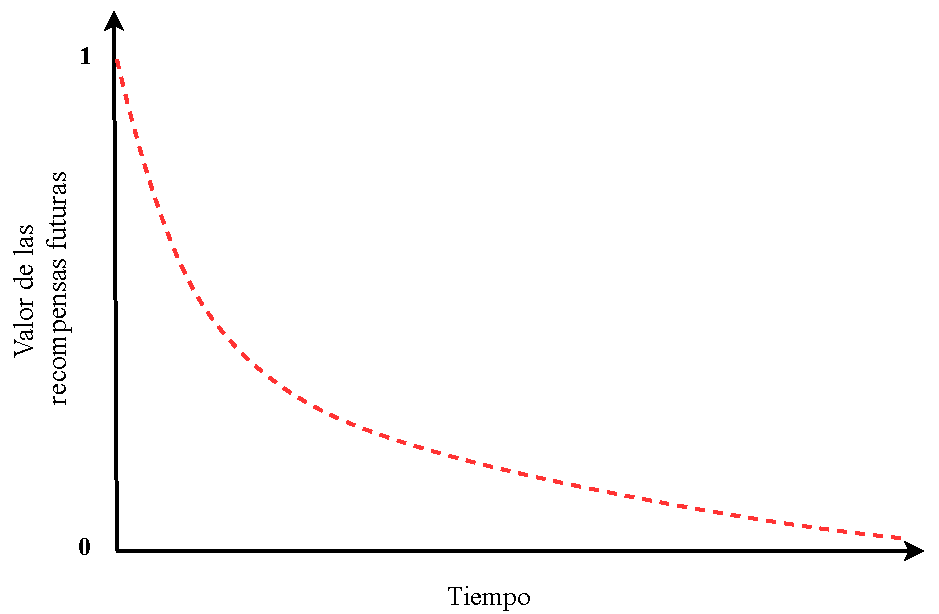
\includegraphics[width=0.9\textwidth]{imagenes/discount.pdf}
    \caption{Influencia del factor de descuento y el tiempo en el valor de las recompensas futuras}
    \label{fig:discount}
\end{figure}

Otra posible definición de la recompensa acumulada es la siguiente formulación recursiva:

\begin{equation}
    G_t \doteq R_{t+1} + \gamma G_{t+1}
\end{equation}

De esta forma, hemos definido los principales elementos que componen un MPD, contando con un modelo de entorno sobre el que un agente puede desenvolverse.

\subsection{Políticas y funciones de valor}

Una vez contamos con el modelo necesario para formular un problema de RL, es momento de abordar su resolución. Buscamos conocer la secuencia de acciones que maximice la recompensa acumulada al final de un episodio. Es aquí donde entra en juego el concepto de \textbf{política}, la cual, como ya adelantábamos, regirá el comportamiento del agente. 

Formalmente, una política es una función $\pi(a|s)$ que refleja la probabilidad de emplear una determinada acción $a \in \mathcal{A}(s)$ si el agente se encuentra actualmente en el estado $s \in \mathcal{S}$. En caso de tratarse de una política \textbf{determinista}, la acción devuelta por $\pi$ será siempre única ($probabilidad = 1$), mientras que, en caso de contar con una política \textbf{estocástica}, tendremos como salida la distribución de probabilidades de todas las acciones posibles.

Un ejemplo muy simple de política puede ser una \textit{función aleatoria}, la cual asigna la misma probabilidad a todas las acciones posibles partiendo del estado actual. Por lo general, una política aleatoria difícilmente permitirá maximizar la recompensa acumulada, al no verse guiada por los \textbf{objetivos} del agente. Un comportamiento más deseable sería, por ejemplo, asignar una mayor probabilidad a aquellas acciones que conduzcan a un estado más favorable y, por tanto, asociado a una mayor recompensa inmediata. Para lograrlo, será necesario definir una serie de funciones que permitan guiar al agente en la maximización de dicha recompensa. Definimos así las funciones \textit{estado-valor} y \textit{acción-valor}:

\begin{itemize}
    \item \textbf{Función estado-valor}, $v_\pi(s)$. Devuelve la recompensa esperada tras aplicar $\pi$ desde el estado $s$. Esto es:
    
    \begin{equation}
        v_\pi(s) \doteq \mathds{E}_\pi [G_t | S_t = s]
    \end{equation}
    
    Nótese cómo, de haberlo, el valor del estado terminal será siempre 0.
    
    \item \textbf{Función acción-valor}, $q_\pi(s,a)$. Devuelve la recompensa esperada tras aplicar la acción $a$ a partir de un estado $s$ siguiendo la política $\pi$. Se define tal que:
    
    \begin{equation}
        q_\pi(s,a) \doteq \mathds{E}_\pi [G_t | S_t = s, A_t = a]
    \end{equation}
\end{itemize}

Tanto $v_\pi$ como $q_\pi$ pueden estimarse a partir de la experiencia. Por ejemplo, un agente que sigue una política $\pi$ puede ir manteniendo la media de las recompensas obtenidas a partir de cada estado, de tal forma que $v_\pi(s)$ acabará convergiendo en el valor real de cada estado. Lo mismo ocurre para $q_\pi$ si se mantiene la recompensa media obtenida a partir de cada combinación estado-acción.

Visto en qué consiste la función \textit{estado-valor}, podemos desarrollarla recursivamente, dando lugar a la conocida como \textbf{ecuación de Bellman} \cite{bellman1966dynamic}:

\begin{equation}
    \begin{split}
        v_\pi(s) & \doteq \mathds{E}_\pi [G_t | S_t = s] \\
        & = \mathds{E}_\pi [R_{t+1} + \gamma G_{t+1} | S_t = s] \\ 
        &= \sum_{a} \pi(a|s) \sum_{s'}\sum_{r} p(s',r|s,a)[r + \gamma \mathds{E}_\pi [G_{t+1} | S_{t+1} = s']] \\ 
        & = \sum_{a} \pi(a|s) \sum_{s',r} p(s',r|s,a)[r + \gamma v_\pi(s')], \forall s \in \mathcal{S}
    \end{split}
\end{equation}

La ecuación de Bellman es un principio fundamental de la programación dinámica \cite{bellman1966dynamic} que expresa la relación entre el valor de un estado y el de sus sucesores. Concretamente, parte del promedio ponderado de todas las probabilidades de transición desde un estado inicial $s$, y establece que el valor de $s$ debe ser igual al valor descontado del siguiente estado esperado, más la recompensa esperada en el resto de la trayectoria a seguir.

El mismo principio puede aplicarse para la función \textit{acción-valor}, dando lugar a:

\begin{equation}
    \begin{split}
        q_\pi(s,a) & \doteq \mathds{E}_\pi [G_t | S_t = s, A_t = a] \\
        & = \mathds{E}_\pi [R_{t+1} + \gamma G_{t+1} | S_t = s, A_t = a] \\ 
        & = \sum_{s', r}p(s',r|s,a)[r + \gamma v_\pi(s')], \forall s \in \mathcal{S}, \forall a \in \mathcal{A}(s)
    \end{split}
\end{equation}

Una vez visto en qué consisten las políticas y funciones \textit{estado-valor} y \textit{acción-valor}, estas podrán servirnos para describir, evaluar y mejorar el comportamiento de los agentes. Como ya hemos indicado, el objetivo de un agente de RL es aspirar al \textbf{comportamiento óptimo} dentro de su entorno. Esta \textit{optimalidad} nos conduce a la definición de los siguientes términos:

\begin{itemize}
    \item \textbf{Política óptima}, $\pi_*$: aquella que, para cada estado, puede obtener recompensas esperadas mayores o iguales a las de cualquier otra política. Podemos comparar políticas en base a sus funciones \textit{estado-valor}:
    
        \begin{equation}
            \label{policy-comparison}
            \pi \geq \pi' \leftrightarrow v_\pi(s) \geq v_{\pi'}(s)
        \end{equation}
        
    De tal forma que la política óptima será aquella tal que:
    
        \begin{equation}
            \pi_* \geq \pi', \forall \pi'
        \end{equation}
   
    \item \textbf{Función \textit{estado-valor} óptima}, $v_*$: función \textit{estado-valor} que ofrece el máximo valor de todas las políticas para todos los estados.
    
        \begin{equation}
            v_*(s) = \underset{\pi}{max}\ v_\pi(s), \forall s \in S
        \end{equation}
    
    \item \textbf{Función \textit{acción-valor} óptima}, $q_*$: función \textit{acción-valor} que ofrece el máximo valor de todas las políticas para todo par \textit{estado-acción}.
    
        \begin{equation}
            q_*(s, a) = \underset{\pi}{max}\ q_\pi(s, a), \forall s \in S, \forall a \in \mathcal{A}(s)
        \end{equation}
\end{itemize}

Finalmente, cabe destacar que, mientras múltiples políticas óptimas pueden coexistir para un mismo MDP, únicamente existirá una única función \textit{estado-valor} y \textit{acción-valor} óptimas.

\subsection{Evaluación y mejora de las políticas}

Llegados a este punto, contamos con las herramientas necesarias para poder \textit{evaluar} políticas y funciones de valor, así como para calcular las funciones de valor y políticas óptimas.

El algoritmo de \textbf{evaluación iterativa de la política} (\textit{iterative policy evaluation}, o simplemente \textit{policy evaluation}) nos permite conocer cómo de ``buena'' o ``mala'' es una política cualquiera en base a su recompensa acumulada esperada. Este algoritmo (ver Algoritmo \ref{alg:policy-eval}, \cite{sutton2018reinforcement}) permite la aproximación iterativa de la función \textit{estado-valor} de la política evaluada a partir de la fórmula:

\begin{equation}
    v_{k+1}(s) =  \sum_{a} \pi(a|s) \sum_{s',r} p(s',r|s,a)[r + \gamma v_k(s')]
\end{equation}

\begin{algorithm}
\caption{Evaluación iterativa de la política}
\label{alg:policy-eval}
\DontPrintSemicolon
\LinesNumbered
\KwIn{$\pi$: la política a evaluar \newline
      $\mathcal{S}$: el espacio de estados del problema \newline
      $\gamma$: el factor de descuento \newline
      $\theta$: un umbral de convergencia}
\KwOut{$V$: los valores finales asociados a cada estado}

    $V(s) = 0, \forall s \in \mathcal{S}+$\;
    $V(terminal) = 0$\;
    
    \Repeat{$\Delta < \theta$}{
        $\Delta \leftarrow 0$\;
        \ForEach{$s \in \mathcal{S}$}{
            $v \leftarrow V(s)$\;
            $V(s) \leftarrow \sum_{a} \pi(a|s) \sum_{s',r} p(s',r|s,a)[r + \gamma V(s')]$\;
            $\Delta \leftarrow max(\Delta, |v-V(s)|)$\;
        }
    }
    
    \Return{V}

\end{algorithm}

donde los valores de los estados convergen cuando $k$ tiende a infinito. 

Una vez sabemos cómo \textit{evaluar} políticas, podemos compararlas entre sí, tal y como se mostró en \ref{policy-comparison}. De hecho, ahora somos capaces de partir de una política cualquiera y tratar de \textit{mejorarla} iterativamente a partir de la función \textit{acción-valor}. Para ello emplearemos el algoritmo de \textbf{mejora iterativa de la política} (ver Algoritmo \ref{alg:policy-impro}, \cite{sutton2018reinforcement}), el cual se define mediante la siguiente fórmula:

\begin{equation}
    \pi'(s) = \underset{a}{argmax}\ \sum_{s',r}p(s', r | s, a)[r + \gamma v_\pi(s')]
\end{equation}

Este algoritmo parte de la estimación de las recompensas para cada acción, $a$, desde el estado actual, $s$, y busca aquellas acciones que conducen al agente a estados sucesores, $s'$, con la máxima estimación \textit{estado-valor}.

\begin{algorithm}
\caption{Mejora iterativa de la política}
\label{alg:policy-impro}
\DontPrintSemicolon
\LinesNumbered
\KwIn{$\pi$: la política a evaluar \newline
      $\mathcal{S}$: el espacio de estados del problema \newline
      $\gamma$: el factor de descuento}
\KwOut{$V_*$: los valores finales asociados a cada estado \newline
       $\pi_*$: la política óptima obtenida}

    $politica\_estable \leftarrow verdadero$\;
    \ForEach{$s \in S$}{
        $a_0\leftarrow \pi(s)$\;
        $\pi(s) \leftarrow \underset{a}{argmax}\ \sum_{s',r}p(s', r | s, a)[r + \gamma V(s')]$\;
        \If{$a_0 \neq \pi(s)$}{
            $politica\_estable \leftarrow falso$\;
        }
    }
    \If{$politica\_estable$}{
        \Return{$V \approx v_*$ y $\pi \approx \pi_*$}\;
    }
    \Else{
        aplicar \textbf{evaluación de la política} y repetir\;
    }

\end{algorithm}

Si combinamos los procesos de evaluación y mejora de la política de forma cíclica, estaremos mejorando $\pi$ iterativamente. Es lo que se denomina \textbf{iteración de la política} (\textit{policy iteration}), consistente en alternar \textit{evaluación} y \textit{mejora} hasta converger en la política óptima ($\pi \approx \pi_*$).

Una solución alternativa a la iteración de la política es el algoritmo de \textbf{iteración de valor} (\textit{value iteration}), consistente en (ver Algoritmo \ref{alg:value-iter}):

\begin{enumerate}
    \item Encontrar la función \textit{estado-valor} óptima, $v_*$. El algoritmo parte de una función de valor aleatoria que mejora iterativamente hasta alcanzar su valor óptimo.
    \item Extraer la política óptima, $\pi_*$, asociada a $v_*$. Una vez contamos con la función de valor óptima, la política óptima $\pi_*$ será aquella que actúe de forma voraz con respecto a $v_*$.
\end{enumerate}

\begin{algorithm}
\caption{Iteración de valor}
\label{alg:value-iter}
\DontPrintSemicolon
\LinesNumbered
\KwIn{$\pi$: la política a evaluar \newline
      $\mathcal{S}$: el espacio de estados del problema \newline
      $\gamma$: el factor de descuento \newline
      $\theta$: un umbral de convergencia}
\KwOut{$V_*$: los valores finales asociados a cada estado \newline
       $\pi_*$: la política óptima obtenida}

    $V(s) = 0, \forall s \in \mathcal{S}+$\;
    $V(terminal) = 0$\;
    
    \Repeat{$\Delta < \theta$}{
        $\Delta \leftarrow 0$\;
        \ForEach{$s \in \mathcal{S}$}{
            $v \leftarrow V(s)$\;
            $V(s) \leftarrow \underset{a}{max}\ \sum_{s',r} p(s',r|s,a)[r + \gamma V(s')]$\;
            $\Delta \leftarrow max(\Delta, |v-V(s)|)$\;
        }
    }
    
    $\pi_*(s) \leftarrow \underset{a}{argmax} \sum_{s',r}p(s', r | s, a)[r + \gamma V(s')]$\;
    
    \Return{$V_*, \pi_*$}

\end{algorithm}

En la práctica, tal y como se indica en \cite{sutton2018reinforcement}, \textit{policy iteration} converge más rápido que \textit{value iteration} (ya que la política converge más rápido que la función \textit{estado-valor}); no obstante, es computacionalmente más complejo, ya que en cada iteración es necesario tanto evaluar como mejorar la política actual.

\subsection{Exploración y explotación}

Muchos de los problemas reales que podemos tratar de resolver mediante RL suponen espacios de estados y acciones muy grandes (o incluso infinitos). Esto hace que los métodos iterativos previamente mencionados sean inviables, ya que no serían capaces de estimar todos los valores y dar con una política óptima en un tiempo razonable. 

Como veremos más adelante, los métodos de aprendizaje utilizados para resolver este tipo de problemas deben dar cabida, no sólo a aprovechar el conocimiento del que ya dispone el agente tras haber interactuado con el entorno, sino también a tratar de conocerlo mejor a lo largo del tiempo.

Surge, pues, un nuevo problema hasta ahora no contemplado en la interacción del agente con el entorno: el balance entre \textbf{exploración} y \textbf{explotación}. Mientras que la \textit{exploración} hace referencia a transiciones entre estados no óptimas destinadas a conocer mejor el entorno, la \textit{explotación} tiene como fin maximizar la recompensa a partir del conocimiento sobre los estados y la política actual del agente.

Cuando un agente explora, ``sacrifica'' recompensas óptimas inmediatas en pos de descubrir nuevas trayectorias que puedan mejorar sus resultados futuros. No obstante, un agente que únicamente explora el entorno difícilmente convergerá en una buena solución, ya que nunca tomará las acciones que maximicen la recompensa. Es necesario, por tanto, buscar un equilibrio entre \textit{exploración} y \textit{explotación} que permita conocer el entorno de forma progresiva pero sin descuidar la acumulación de recompensas.

Existen diferentes formas de afrontar este equilibrio. Por ejemplo, el método $\epsilon$-\textit{greedy} se basa en actuar siguiendo una estrategia voraz (\textit{greedy}), pero permitiendo tomar acciones aleatorias bajo cierta probabilidad $\epsilon$. Dichas acciones aleatorias suponen \textit{explorar} en lugar de \textit{explotar}.

Finalmente, existen otras estrategias que consideran y/o codifican el factor de incertidumbre de los diferentes estados, de tal forma que, a medida que crece la incertidumbre sobre un estado, mayor probabilidad habrá de transitar hacia él.

\subsection{Algoritmos clásicos de RL}

Hasta el momento, hemos visto cómo emplear \textit{iteración de la política} e \textit{iteración de valor} para extraer la política óptima asociada a un MDP. Decimos, por tanto, que son \textbf{métodos dependientes del modelo} del entorno (\textit{model-based}). Concretamente, las funciones de transición y recompensa son las que definen las dinámicas del entorno, y las empleadas por estos métodos para optimizar la política empleada. Así, la principal ventaja de los métodos basados en modelos es que los estados futuros y las recompensas pueden anticiparse a través del modelo del entorno, lo que permite al agente a lograr una mejor planificación \cite{zhang2020taxonomy}.

No obstante, en la mayoría de problemas reales carecemos de un modelo que nos permita conocer de forma anticipada las dinámicas del entorno, ya sea por complejidad o por falta de información\footnote{Por ejemplo, podría darse el caso de que no se cumpliese la propiedad de Markov.}. Ante esta problemática, surgen los \textbf{métodos libres de modelo}, o \textit{model free}, los cuales estiman la función de valor y la política a partir de la experiencia. Estos modelos son más cercanos a la esencia de aprendizaje por refuerzo, ya que dependen exclusivamente del ensayo-error para aprender el comportamiento óptimo\footnote{Es lo que se denomina un \textit{problema de control}, en contraposición a los \textit{problemas de predicción} ya vistos, donde el objetivo era evaluar políticas o estimar funciones de valor dada una política. La resolución de un \textit{problema de control} consiste en optimizar de forma progresiva las estimaciones de la función \textit{acción-valor} \cite{morales2020grokking}.}. A continuación, estudiaremos en detalle su funcionamiento.

\subsubsection{Monte Carlo}

Los algoritmos de tipo \textbf{Monte Carlo} (MC) consisten en la ejecución de múltiples episodios que permitan recopilar diferentes trayectorias a lo largo del espacio de estados y acciones. De esta forma, el valor de cada estado será el promedio de las recompensas acumuladas en cada \textit{visita}. La misma filosofía puede aplicarse para estimar el valor de los pares estado-acción, especialmente si no disponemos de un modelo del entorno. Así, una vez conocido el valor de cada estado, o par acción-estado, podremos extraer la política óptima.

Nótese cómo, a medida que se simule un mayor número de episodios, el promedio de las recompensas para cada estado, $s$, tenderá a converger en $v_\pi(s)$. Lo mismo ocurrirá en el caso de los pares estado-acción, con tendencia a $q_\pi(s,a)$.

Uno de los problemas que pueden darse a la hora de calcular el promedio de las recompensas es que un estado (o par estado-acción) sea visitado múltiples veces en un mismo episodio. Ante esta situación, podemos considerar únicamente el valor obtenido en la primera visita (\textit{first-visit MC}; ver Algoritmo \ref{alg:first-MC}) o calcular la media de las recompensas obtenidas (\textit{every-visit MC}).

\begin{algorithm}
\caption{\textit{First-visit} MC, \cite{zhang2020taxonomy}}
\label{alg:first-MC}
\DontPrintSemicolon
\LinesNumbered
\KwIn{$\pi$: la política a evaluar}

Inicializar arbitrariamente $V(s), \forall s \in \mathcal{S}$\;
$recompensas(s) \leftarrow \{ \}, \forall s \in \mathcal{S}$\;

    \Repeat{no haya convergencia}{
        Generar un episodio siguiendo $\pi$: $S_0, A_0, R_1, S_1, A_1, R_2, ..., S_{T-1}, A_{T-1}, R_T$\;
        $G \leftarrow 0$\;
        $t \leftarrow T -1$\;
        \ForEach{paso en el episodio, $t = T - 1, T - 2, ... 0$}{
            $G \leftarrow \gamma G + R_{t+1}$\;
            \If{$S_0, S_1, ..., S_{t-1}$ no contiene a $S_t$}{
                $recompensas(S_t) \leftarrow recompensas(S_t) \cup \{G\}$
                $V(S_t) \leftarrow mean(recompensas(S_t))$\;
            }
        }
    }
\end{algorithm}

La exploración sigue siendo un factor importante, ya que adherirnos estrictamente a una política $\pi$ podría impedirnos conocer trayectorias que afecten a las estimaciones obtenidas. Es aconsejable, por tanto, seguir una política similar a $\epsilon$-\textit{greedy} que dé cabida a dicha exploración. De hecho, el valor de $\epsilon$ no tiene por qué ser estático, pudiendo ir reduciéndose a lo largo del tiempo, de tal forma que la exploración disminuya a medida que los valores estimados converjan \cite{morales2020grokking}.

Finalmente, aunque los algoritmos de tipo MC son sencillos y eficaces, también presentan ciertos problemas, tales como la necesidad de esperar a la finalización de cada episodio para actualizar los valores estimados, una alta variabilidad en las estimaciones, o tiempos de ejecución muy elevados para poder alcanzar la convergencia en entornos complejos.

\subsubsection{Diferencia temporal}

El aprendizaje por \textbf{diferencia temporal} (\textit{temporal-difference}, TD) es uno de los principales cimientos del aprendizaje por refuerzo, el cual combina ideas de los métodos basados en Monte Carlo y programación dinámica \cite{sutton2018reinforcement}. Además, constituye la base de algunos de los métodos que estudiaremos más adelante.

Tanto TD como Monte Carlo son métodos libres de modelo basados en la experiencia. En el caso de Monte Carlo, es necesario esperar a la finalización del episodio para calcular $V(S_t)$, ya que la estimación del valor de un estado depende de las estimaciones de todos los estados futuros visitados hasta obtener $G_t$. Veamos como representarlo formalmente:

\begin{itemize}
    \item Partimos de la idea de que la media $\mu_1, \mu_2, ..., \mu_n$ de una secuencia $x_1, x_2, ..., x_n$ puede calcularse de forma incremental de la siguiente forma:

    \begin{align}
        \mu_k = & \frac{1}{k} \sum_{j=1}^{k} x_j \\
              = & \frac{1}{k} (x_k + \sum_{j=1}^{k-1} x_j) \\
              = & \frac{1}{k} (x_k + (k-1)\mu_{k-1}) \\
              = & \mu_{k-1} + \frac{1}{k}(x_k - \mu_{k-1})
    \end{align}
    
    \item Cuando seguimos un método basado en MC, podemos aplicar esta idea para actualizar de forma incremental el valor de cada estado tras un episodio. De esta forma, para cada estado $S_t$, dada una recompensa final $G_t$:
    
    \begin{gather}
        N(S_t) \leftarrow N(S_t) + 1 \\
        V(S_t) \leftarrow V(S_t) + \frac{1}{N(S_t)}(G_t - V(S_t))
    \end{gather}
    
    O, de forma general:
    
    \begin{equation}
        V(s_{t+1}) \leftarrow V(s_t) + \alpha[objetivo - V(s_t)]
    \end{equation}
    
    siendo $\alpha$ un parámetro que representa el ``tamaño de paso'', o \textit{step-size}, y \textit{objetivo} la n-ésima recompensa obtenida\footnote{A la expresión $[objetivo - v(s_t)]$ se le denomina \textit{error de la estimación}, y se reduce conforme nos acercamos al \textit{objetivo}.}. 
    
    \item En el caso de MC, el objetivo es la recompensa final ($objetivo = G_t$). Esto, finalmente, nos lleva al cálculo incremental de $V(s_t)$:

    \begin{equation}
        V(S_t) \leftarrow V(S_t) + \alpha [G_t - V(S_t)]
    \end{equation}
    
    Podemos ver cómo los métodos basados en MC dependen de $G_t$ para actualizar el valor de los estados, lo que supone esperar a la finalización del episodio completo para actualizar dichas estimaciones.
\end{itemize}

A diferencia de Monte Carlo, TD no necesita esperar a conocer la recompensa final, $G_t$, para actualizar $V(s_t)$, sino únicamente esperar al siguiente \textit{paso}, $t+1$. Esto es:

\begin{equation}
    V(S_t) \leftarrow V(S_t) + \alpha[R_{t+1} + \gamma V(S_{t+1}) - V(S_t)]
\end{equation}

En este caso, $objetivo = R_{t+1} + \gamma V(S_{t+1})$, ya que se considera la recompensa $R_{t+1}$ y la estimación $V(S_{t+1})$ del siguiente \textit{timestep}\footnote{En este caso, $R_{t+1} + \gamma V(S_{t+1})$ es el \textit{objetivo} (\textit{TD target}), mientras que $R_{t+1} + \gamma V(S_{t+1}) - V(S_t)$ es el \textit{error} (TD error).}$^,$\footnote{Nótese cómo el valor de $\alpha$ pondera la importancia relativa de la nueva estimación de valor frente a la actual. Si $\alpha = 1$, se ignora la estimación previa, mientras que, si $\alpha = 0$, no se produce ninguna actualización.}. Es lo que denominamos $TD(0)$, o \textit{one-step TD} (ver Algoritmo \ref{alg:td}), el cual es un caso especial de \textit{n-step TD}:

\begin{equation}
    V_{t+n}(S_t) = V_{t+n-1}(S_t) + \alpha(G_{t:t+n} - V_{t+n-1}(S_t)
\end{equation}

Siendo $G_{t:t+n}$ la recompensa obtenida desde el instante $t$ hasta $t+n$; esto es: $R_{t+1} + \gamma R_{t+2} + ... + \gamma^{n-1} R_{t+n} + \gamma^n V_{t+n-1}(S_{t+n})$.

\begin{algorithm}
\caption{$TD(0)$, \cite{sutton2018reinforcement}}
\label{alg:td}
\DontPrintSemicolon
\LinesNumbered
\KwIn{$\pi$: la política a evaluar \newline
     $\alpha$: el \textit{step-size} $\in (0,1]$}

Inicializar arbitrariamente $V(s), \forall s \in \mathcal{S^+}$\;
$V(terminal) = 0$\;

 \ForEach{episodio}{
    Inicializar $S$\;
    \Repeat( para cada \textit{paso} en el episodio:){$S$ no sea terminal}{
        $A \leftarrow \pi(S)$\;
        Realizar acción $A$ y observar $R, S'$\;
        $V(S) \leftarrow V(S) + \alpha[R + \gamma V(S') - V(S)]$\;
        $S \leftarrow S'$\;
    }
 
 }
\end{algorithm}

En caso de utilizar \textit{n-step TD}, se nos plantea el interrogante de qué valor de $n$ utilizar. De hecho, podríamos plantear la posibilidad de combinar la información de múltiples \textit{timesteps} (por ejemplo, tomar como valores las medias de las estimaciones entre TD(2) y TD(4)) o incluso de todos ellos, asignando una mayor importancia a aquellos valores estimados más cercanos en el tiempo. Así surge el algoritmo $TD(\lambda)$, donde la recompensa $G^\lambda_t$ combina todas las recompensas en $G^{(n)}_t$, asignando una ponderación $(1-\lambda)\lambda^{n-1}$ a cada una de ellas. Esto es:

\begin{equation}
    G^\lambda_t = (1-\lambda) \sum^{\infty}_{n=1}\lambda^{n-1} G^{(n)}_t
\end{equation}

Así, $TD(\lambda)$ generaliza los métodos vistos hasta el momento, ya que equivale a Monte Carlo cuando $\lambda = 1$, y a $TD(0)$ cuando $\lambda = 0$. Existen, a su vez, dos formas de aplicar $TD(\lambda)$: hacia delante (\textit{forward-view}) o hacia atrás (\textit{backward-view}) \cite{morales2020grokking}:

\begin{itemize}
    \item \textit{Forward-view} $TD(\lambda)$: combina $n$ pasos en una sola actualización. El agente debe esperar hasta el final del episodio antes de poder actualizar las estimaciones.
    \item \textit{Backward-view} $TD(\lambda)$: divide las actualizaciones de los valores en actualizaciones parciales, que aplica en cada paso. Emplea rastros de elegibilidad (\textit{eligibility traces}) para decidir qué estados actualizar.
\end{itemize}

A modo de conclusión, TD es capaz de aprender a partir de episodios incompletos, actualizando estimaciones de valor en base a otras estimaciones de valor (es lo que se denomina \textit{bootstrapping}). Esto supone ciertas ventajas con respecto a MC, ya que:

\begin{itemize}
    \item TD puede aprender de forma \textit{online}, mientras que MC debe esperar al final del episodio hasta conocer la recompensa final obtenida.
    \item TD presenta una menor variabilidad en las estimaciones con respecto a MC.
    \item TD puede aprender a partir de secuencias incompletas, mientras que MC solamente aprende a partir de episodios completos.
    \item TD funciona en entornos continuados donde no existe un estado terminal, mientras que MC únicamente funciona en entornos episódicos.
\end{itemize}

Finalmente, cabe destacar cómo MC presenta un menor sesgo (\textit{bias}) en las estimaciones, ya que los valores se actualizan directamente en base a la recompensa final, y no con respecto a otras predicciones, como ocurre en el caso de TD.

\subsubsection{SARSA}

Una vez hemos visto como utilizar TD para resolver el problema de \textit{predicción}, estudiaremos cómo utilizarlo en \textit{control}. Partimos de la idea de que TD puede emplearse para calcular $q_\pi(s,a)$ de la misma forma que hicimos con $v_\pi(s,a)$:

\begin{equation}
    Q(S_t, A_t) \leftarrow Q(S_t, A_t) + \alpha \left [R_{t+1} + \gamma Q(S_{t+1}, A_{t+1}) - Q(S_t, A_t) \right ]
\end{equation}

Esta actualización se produce en cada transición desde estados no terminales $S_t$. Así, en caso de que $S_{t+1}$ sea terminal, $Q(S_{t+1}, A_{t+1}) = 0$. 

Podemos observar cómo el uso de cada uno de los elementos de la quíntupla $(S_t, A_t, R_{t+1}, S_{t+1}, A_{t+1})$ da lugar al nombre de este algoritmo: \textbf{SARSA} (ver Algoritmo \ref{alg:sarsa}).

\begin{algorithm}
\caption{SARSA (\textit{on-policy TD control)}, \cite{sutton2018reinforcement}}
\label{alg:sarsa}
\DontPrintSemicolon
\LinesNumbered
\KwIn{$\alpha$: el \textit{step-size} $\in (0,1]$ \newline
      $\epsilon > 0$}

Inicializar arbitrariamente $Q(s, a), \forall s \in \mathcal{S^+}, \ a \in \mathcal{A}(s)$\;
$Q(terminal, \cdot) = 0$\;

 \ForEach{episodio}{
    Inicializar $S$\;
    Elegir $A$ desde $S$ empleando una política derivada de $Q$ (por ejemplo, $\epsilon$-greedy)\;
    \Repeat( para cada \textit{paso} en el episodio:){$S$ no sea terminal}{
        Realizar acción $A$ y observar $R, S'$\;
        $Q(S,A) \leftarrow Q(S,A) + \alpha[R + \gamma Q(S',A') - Q(S,A)]$\;
        $S \leftarrow S'$; $A \leftarrow A'$\;
    }

 }
\end{algorithm}

Al igual que en el caso de TD, SARSA puede emplearse siguiendo un enfoque \textit{n-step}, dando lugar a \textit{n-step SARSA}, en contraposición a \textit{one-step SARSA} o \textit{SARSA(0)}. En este caso, la regla de actualización empleada es la siguiente:

\begin{equation}
    Q_{t+n}(S_t, A_t) = Q_{t+n-1}(S_t, A_t) + \alpha \left [G_{t:t+n} + \gamma Q_{t+n-1}(S_t, A_t) \right ]
\end{equation}

Llegados a este punto, es necesario diferenciar entre dos tipos de métodos: \textbf{on-policy} y \textbf{off-policy}:

\begin{itemize}
    \item Los métodos \textit{on-policy} estiman la recompensa $Q(s,a)$ asociada a cada par acción-estado asumiendo que se continuará siguiendo la política actual.
    \item Por otro lado, los métodos \textit{off-policy} actualizan el valor de cada par acción-estado asumiendo que posteriormente se seguirá una política voraz. De esta forma, la política actualizada es diferente a la que se asume que será seguida\footnote{Nótese cómo, en caso de seguir una política voraz, la distinción entre \textit{on-policy} y \textit{off-policy} desaparece.}.
\end{itemize}

Por tanto, decimos que SARSA es un método \textit{on-policy} porque la política que se utiliza para actualizar las estimaciones y la que se utiliza para actuar es la misma. 

\subsubsection{Q-learning}

Una alternativa \textit{off-policy} a SARSA es \textbf{Q-learning} \cite{watkins1992q}, un algoritmo de control de especial relevancia en el campo del aprendizaje por refuerzo. Decimos que Q-learning es un algoritmo \textit{off-policy} porque la política actualizada es diferente de la política de comportamiento:

\begin{itemize}
    \item La \textbf{política de comportamiento} (\textit{behavior policy}) se emplea para generar interacciones con el entorno.
    \item Por otro lado, la \textbf{política objetivo} (\textit{target policy}) es la política que el agente aprende.
\end{itemize}

La ecuación empleada por Q-learning para actualizar las estimaciones de cada par acción-estado es la siguiente (ver Algoritmo \ref{alg:qlearning}):

\begin{equation}
    Q(S_t, A_t) \leftarrow Q(S_t, A_t) + \alpha[R_{t+1} + \gamma\ \underset{a}{max}\ Q(S_{t+1}, a) - Q(S_t, A_t)]
\end{equation}

\begin{algorithm}
\caption{Q-learning (\textit{off-policy TD control)}, \cite{sutton2018reinforcement}}
\label{alg:qlearning}
\DontPrintSemicolon
\LinesNumbered
\KwIn{$\alpha$: el \textit{step-size} $\in (0,1]$ \newline
      $\epsilon > 0$}

Inicializar arbitrariamente $Q(s, a), \forall s \in \mathcal{S^+}, \ a \in \mathcal{A}(s)$\;
$Q(terminal, \cdot) = 0$\;

 \ForEach{episodio}{
    Inicializar $S$\;
    Elegir $A$ desde $S$ empleando una política derivada de $Q$ (por ejemplo, $\epsilon$-greedy)\;
    \Repeat( para cada \textit{paso} en el episodio:){$S$ no sea terminal}{
        Realizar acción $A$ y observar $R, S'$\;
        $Q(S, A) \leftarrow Q(S, A) + \alpha[R + \gamma\ \underset{a}{max}\ Q(S', a) - Q(S, A)]$\;
        $S \leftarrow S'$
    }

 }
\end{algorithm}

A diferencia de SARSA, Q-learning aprende una función acción-valor, $Q$, que se aproxima directamente a la función acción-valor óptima, $q_*$, independientemente de la política seguida. Así, Q-learning siempre convergerá en la política óptima.

Finalmente, desde un punto de vista computacional, lo habitual es representar los valores de cada par acción-estado a partir de una tabla $Q$ que se actualiza siguiendo el proceso mostrado en la Figura \ref{fig:qlearning}.

\begin{figure}
    \centering
    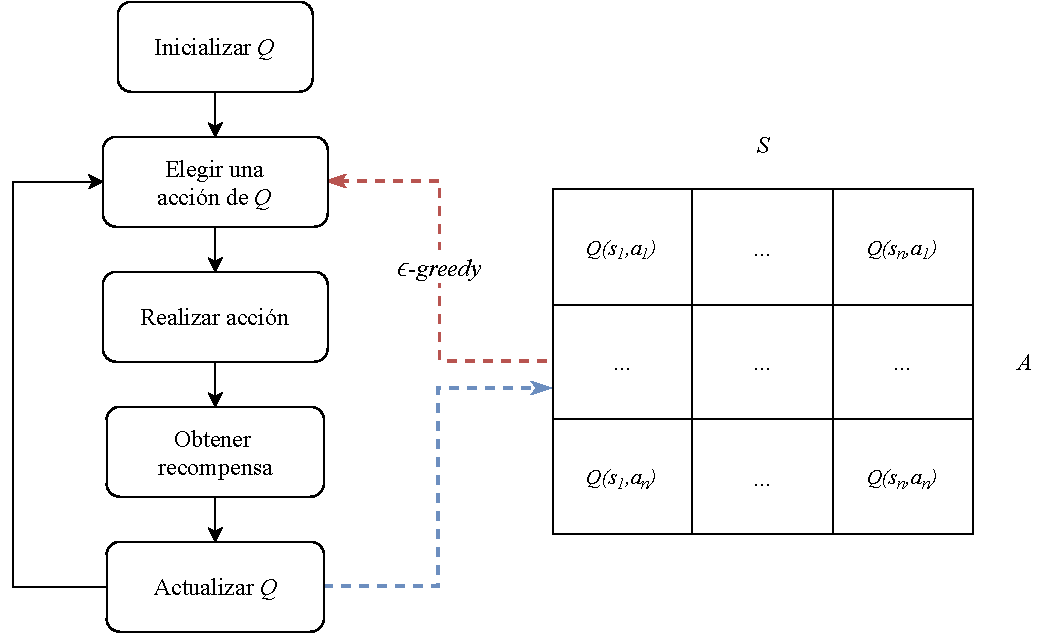
\includegraphics[width=\textwidth]{imagenes/qlearning.pdf}
    \caption{Entrenamiento mediante Q-learning}
    \label{fig:qlearning}
\end{figure}

\subsection{\textit{Deep Reinforcement Learning}}

Hasta el momento, hemos estudiado una serie algoritmos de RL ``clásicos'' capaces de ofrecer muy buenos resultados en entornos de baja complejidad. Simplemente actualizando de forma iterativa una tabla (\textit{lookup table} o \textit{memory table}) con diferentes estados, acciones y recompensas ha sido posible optimizar el comportamiento de un agente. No obstante, estos \textit{métodos tabulares} comienzan a ser inviables a medida que la complejidad de los entornos crece \cite{zai2020deep}. Dicho aumento en la complejidad puede venir dado por un considerable crecimiento en el número de acciones o estados que conforman el entorno, el cual puede tratar de paliarse con métodos \textit{ad hoc} difícilmente generalizables. Por ejemplo, un agente de RL que trabaja con imágenes podría adaptarse para únicamente atender a determinadas porciones de las mismas, en vez de utilizar todos los píxeles que las componen para definir un estado. De esta forma, estaríamos simplificando el espacio de estados, pero la solución propuesta podría no ser válida para otros problemas basados en imágenes donde las regiones a observar sean diferentes.

Ante este tipo de problemas, sería deseable contar con cierta capacidad de abstracción, permitiendo extraer la importancia de las diferentes características que definen un estado. Es aquí donde entra en juego el \textbf{aprendizaje profundo} (\textit{Deep Learning}, DL). En los últimos años, la combinación de RL con redes neuronales profundas ha dado lugar a lo que conocemos como \textbf{aprendizaje profundo por refuerzo} (\textit{Deep Reinforcement Learning}, DRL), el cual ha abierto la puerta a numerosas aplicaciones del aprendizaje por refuerzo en entornos reales. Así, los algoritmos de DRL combinan lo mejor de ambos mundos, dotando al aprendizaje por refuerzo de poder de representación, eficiencia y flexibilidad del aprendizaje profundo \cite{zai2020deep}.

En las siguientes subsecciones veremos algunos de los algoritmos de DRL más conocidos y empleados en este proyecto, abordando en detalle su funcionamiento y características.

\subsubsection{DQN}

Los algoritmos basados en \textbf{\textit{Deep Q-Networks}} (\textbf{DQN}) supusieron un importante hito en el ámbito del aprendizaje por refuerzo, siendo la primera aproximación a lo que hoy conocemos como DRL \cite{mnih2013playing, mnih2015human}. Se denominan métodos \textbf{basados en valor} (\textit{value-based)}, los cuales se fundamentan en el uso de redes neuronales para aproximar el valor de la función $Q$, que pasa a ser modelada de forma no lineal. De esta forma, sustituyen la tabla empleada por Q-learning por una red neuronal\footnote{Esta red puede ser un perceptrón multicapa (MLP) o, en el caso de trabajar con imágenes como datos de entrada, es común emplear redes neuronales convolucionales (CNN) como preprocesamiento previo al MLP. Un ejemplo muy representativo es el de los agentes entrenados para jugar a juegos de Atari \cite{mnih2013playing}.}, tal y como se muestra en la Figura \ref{fig:dqn}.

\begin{figure}
    \centering
    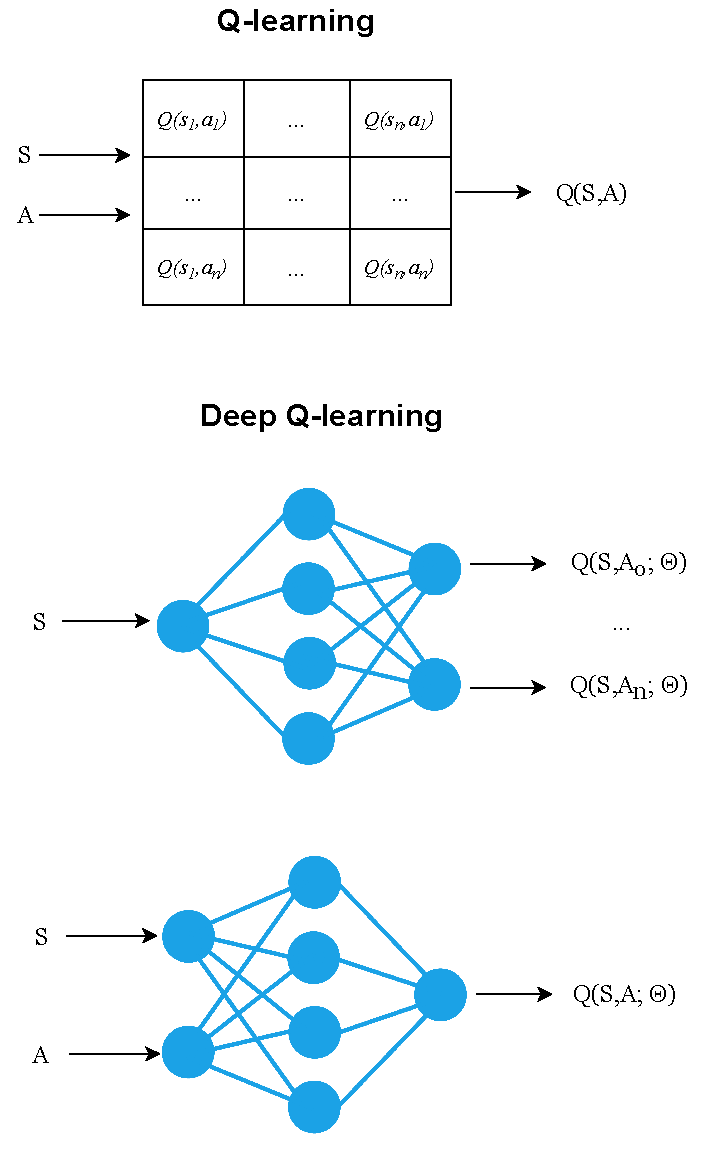
\includegraphics[width=0.7\textwidth]{imagenes/DQN.pdf}
    \caption{Diferencias entre Q-learning y DQN en sus diferentes formulaciones}
    \label{fig:dqn}
\end{figure}

Así, la capa de entrada de la red estará compuesta por tantas neuronas como variables conforman un estado u observación, mientras que las neuronas de salida serán tantas como acciones pueda realizar el agente. En base a la entrada $s$, la siguiente acción a realizar por el agente será la correspondiente a la neurona con mayor valor de salida en la \textit{Q-Network}: $Q(s,a_n;\theta)$, siendo $s$ el estado de entrada, $a_n$ la acción a realizar y $\theta$ el conjunto de pesos de la red\footnote{También es posible dar cabida a la exploración siguiendo una estrategia $\epsilon$-\textit{greedy}.}. Otras formulaciones alternativas permiten tomar pares estado-acción como entrada, para así obtener como salida el valor $Q(s,a; \theta)$ asociado a dicha entrada. Esta última formulación resulta de especial interés en problemas con espacios de acciones continuos, como se verá más adelante. 

Si atendemos a cómo estos sistemas aprenden, la función de pérdida (\textit{loss}) empleada por DQN es el error cuadrático medio (MSE) de la diferencia entre el $Q$-$value$ predicho y el valor objetivo, esto es:

\begin{equation}
    MSE = \mathds{E}_\pi[(Q(S,A) - Q(S,A;\theta))^2]
\end{equation}

Una de las principales limitaciones de DQN es el trabajo con espacios de acciones continuos, ya que al existir infinitas posibilidades no podremos obtener la acción óptima que sirva para computar el error. Dicho problema puede tratar de solventarse considerando como entrada el par $(s,a)$, o directamente discretizando el espacio de acciones, lo cual no deja de ser una limitación para este tipo de algoritmos. Esto lleva a que DQN, por lo general, no sea utilizado con espacios de acciones continuos.

El objetivo será, por tanto, medir la diferencia entre el valor real de $Q$ y el obtenido por la red, para finalmente aplicar descenso del gradiente y optimizar la función de error. La actualización de los pesos de la red se lleva a cabo de acuerdo a:
    
\begin{gather}
    \Delta \Theta = \Delta w = - \eta \frac{\partial E}{\partial w} \\
    \frac{\partial E}{\partial w} = 2(Q(S,A)-Q(S,A;\Theta)) \frac{\partial Q(S,A;\Theta)}{\partial w} \\
    \frac{\partial Q(S,A;\Theta)}{\partial w} = \nabla_\Theta Q(S,A;\Theta) \\
    \Delta \theta = -2 \eta (Q(S,A) - Q(S,A;\Theta)) \nabla_\Theta Q(S,A;\Theta)
\end{gather}

Al no conocer $Q(S,A)$, se aplica la expresión ya vista en Q-learning:

\begin{gather}
    Q(S_0,A_0) \leftarrow Q(S_0,A_0) + \alpha[R_1 + \gamma \ \underset{a \in A}{max} \ Q(S_1,a) - Q(S_0, A_0)] \\
    \Delta \Theta = \alpha [R + \gamma \ \underset{a \in A}{max} Q(S',a;\Theta)-Q(S,A;\Theta)] \nabla_\Theta \ Q(S,A;\Theta)
\end{gather}

Llegados a este punto, un problema que se nos plantea es que la misma red está calculando tanto el valor $Q$ predicho como el valor objetivo. Teniendo en cuenta esto, cuando los pesos se actualicen, los valores $Q$ de salida se actualizarán, pero también lo harán los valores $Q$ objetivo, ya que los objetivos se calculan utilizando los mismos pesos. Así, nuestros valores $Q$ se actualizarán con cada iteración para acercarse a los valores $Q$ objetivo, pero los valores $Q$ objetivo también se moverán en la misma dirección. 

Esto nos lleva a introducir una segunda red que haga el entrenamiento más estable, tal y como se propone en el artículo original \cite{mnih2015human} (ver Figura \ref{fig:dqn-nets}):

\begin{itemize}
    \item Por un lado, la \textbf{red de predicción} (\textit{prediction network}) es la encargada de calcular el valor $Q(S,A;\Theta)$.
    \item Por otro lado, la \textbf{red objetivo} (\textit{target network}) se encarga de estimar el valor objetivo, permitiendo el cálculo del error de forma imparcial. Se sincroniza con la red de predicción cada cierto número de iteraciones, lo que hace que sus pesos se actualicen con menor frecuencia.
\end{itemize}

\begin{figure}
    \centering
    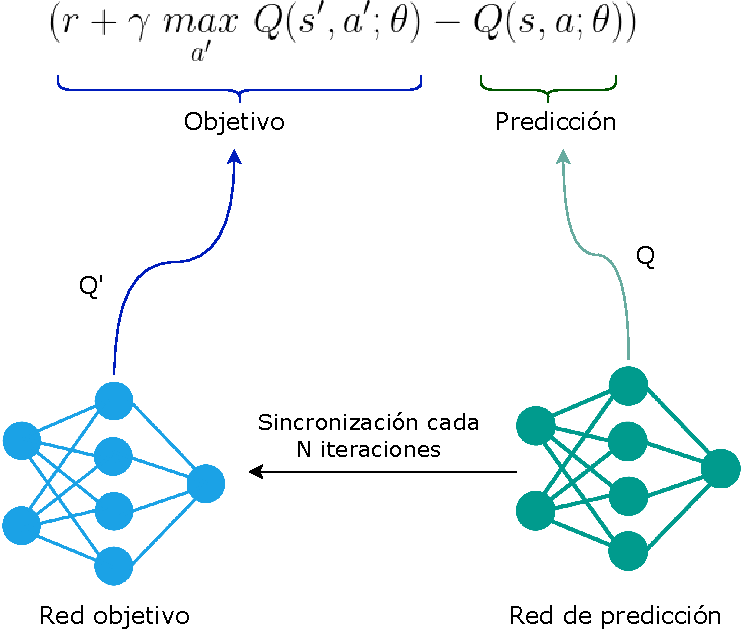
\includegraphics[width=0.8\textwidth]{imagenes/dqn-nets.pdf}
    \caption{Redes empleadas por DQN}
    \label{fig:dqn-nets}
\end{figure}

De forma adicional, es común combinar DQN con una \textbf{memoria de experiencias} que permita almacenar y utilizar como entrada diferentes muestras de experiencias pasadas $(S_t, A_t, R_t, S_{t+1})$ para predecir nuevos valores. Es lo que denominamos \textbf{repetición de la experiencia} \textit{experience replay}.

Finalmente, el proceso de aprendizaje mediante DQN queda resumido en el Algoritmo \ref{alg:dqn}. Cabe destacar la existencia de diferentes variantes de DQN orientadas a mejorar el método original, tales como \textit{Double Q-Learning} \cite{van2016deep}, \textit{Prioritized replay} \cite{schaul2015prioritized} o \textit{Dueling DQN} \cite{wang2016dueling}.

\begin{algorithm}
\caption{DQN}
\label{alg:dqn}
\DontPrintSemicolon
\LinesNumbered
\KwIn{$N$: número de iteraciones necesarias para sincronizar las redes de predicción y objetivo.}

    Inicializar la memoria de experiencias.\;
    Inicializar la red de predicción aleatoriamente.\;
    Crear la red objetivo como una copia de la red de predicción.\;

    $k \leftarrow 0$\;
    
    \ForEach{episodio}{
        
        Inicializar el estado inicial\;
        
        \ForEach{timestep}{
        
            $a \leftarrow$ seleccionar una acción (vía exploración o explotación) en base al valor de $Q$ predicho.\;
            Ejecutar la acción $a$, y observar la recompensa $r$ y el nuevo estado $s'$.\;
            Almacenar la tupla $(s,a,r,s')$ en la memoria de experiencias.\;
            Seleccionar un lote (\textit{batch}) aleatorio de la memoria de experiencias.\;
            Introducir \textit{batch} en la red de predicción\;
            Obtener la salida de la red objetivo para $s'$.\;
            Calcular el error (\textit{loss}) entre los valores $Q$ de salida y objetivo.\;
            Aplicar descenso del gradiente para actualizar los pesos de la red de predicción y reducir el valor de \textit{loss}.\;
            
            \If{$k = N$}{
                Actualizar pesos de la red objetivo con los valores de los pesos de la red de predicción.\;
            }
            
            $k \leftarrow k + 1$\;
        
        }
}

\end{algorithm}

\subsubsection{PPO}

Los métodos basados en \textbf{optimización de la política próxima} (\textit{Proximal Policy Optimization}, o \textbf{PPO}) \cite{schulman2017proximal, hsu2020revisiting} incorporan el gradiente de políticas al aprendizaje por refuerzo. Se trata de un algoritmo \textit{online}, por lo que no emplea una memoria de experiencias. El proceso de aprendizaje es el siguiente:

\begin{enumerate}
    \item Acumular experiencia hasta completar un lote o \textit{batch}.
    \item Utilizar dicha experiencia para optimizar la política.
    \item Descartar el \textit{batch} empleado y volver a 1.
\end{enumerate}

Al tratarse de un método \textit{online}, cada \textit{batch} solamente se emplea una vez para actualizar el gradiente, y después se desecha. Esto lleva a que los métodos basados en gradiente generalmente sean menos eficientes en el aprendizaje con respecto a métodos \textit{offline} como DQN.

Veamos en qué consiste este aprendizaje. PPO está basado en la \textbf{función de acción-ventaja}, la cual determina cómo de buena es una acción $a$ en base a la recompensa que normalmente se espera obtener siguiendo la política $\pi$:

\begin{equation}
\label{advantage}
    a_\pi(s,a) = q_\pi(s,a) - v_\pi(s)
\end{equation}

A partir de esta función acción-ventaja, definimos la función de pérdida como:

\begin{equation}
    L^{PG}(\theta) = \hat{\mathds{E}}_t[log\pi_\theta(a_t|s_t)\hat{A}_t]
\end{equation}

donde $\pi_\theta$ es la política seguida y $\hat{A}_t$ la función acción-ventaja. La idea será favorecer aquellas acciones que lleven a una función de ventaja positiva y, de esta forma, se incrementará la posibilidad de volver a elegir la acción $a$ a partir del estado $s$.

Uno de los principales problemas que supone esta forma de actualizar la política es que puede existir una alta divergencia entre la política original y la actualizada. Para evitar esto, PPO hace uso de \textbf{TRPO}  (\textit{Trust Region Policy Optimization}) y \textbf{KL} (coeficiente de divergencia de Kullback-Leibler) para establecer restricciones de divergencia que permitan que las actualizaciones se realicen únicamente dentro de una ``región de confianza'' \cite{schulman2015trust}. Esto permite que la nueva política obtenida no varíe demasiado con respecto a la anterior. Así, el siguiente ratio:

\begin{equation}
    r(\theta) = \frac{\pi_{\theta_ {old}}(a|s)}{\pi_\theta(a|s)}
\end{equation}

es empleado en la función objetivo de TRPO tal que:

\begin{equation}
    J(\theta)^{TRPO} = E[r(\theta) \hat{A}_{\theta_{old}}(s,a)]
\end{equation}

Si añadimos la restricción que obliga a que este ratio esté entre $1-\epsilon$ y $1+\epsilon$, tenemos la función objetivo empleada por PPO para actualizar la política:

\begin{equation}
    J^{CLIP}(\theta) = \mathds{E}[min(r(\theta)\hat{A}_{\theta_{old}}(s,a), clip(r(\theta), 1-\epsilon, 1+\epsilon)\hat{A}_{\theta_{old}}(s,a)]
\end{equation}

De esta forma, el ratio queda truncado en el rango $[1-\epsilon, 1+\epsilon]$ (mediante la función $clip$), evitando que se produzcan grandes desviaciones en la política, y de tal forma que PPO toma el valor mínimo entre el valor original y el truncado.

\subsubsection{A2C}

El algoritmo \textbf{\textit{Advantage Actor Critic}} (\textbf{A2C}) se encuentra dentro de la familia de métodos \textit{actor-critic} (ver Figura \ref{fig:actor-critic}) en los que una red \textit{actor} se encarga de aprender una política, mientras que otra red  \textit{crítica} se encarga de evaluarla. De esta forma, la red \textit{critic} aprende el valor de los estados, mapeando cada uno con su valor correspondiente. Esta información es empleada por la red \textit{actor} para mejorar el comportamiento, mapeando cada estado con una distribución de probabilidades que indican la preferencia por unas acciones u otras.

\begin{figure}
    \centering
    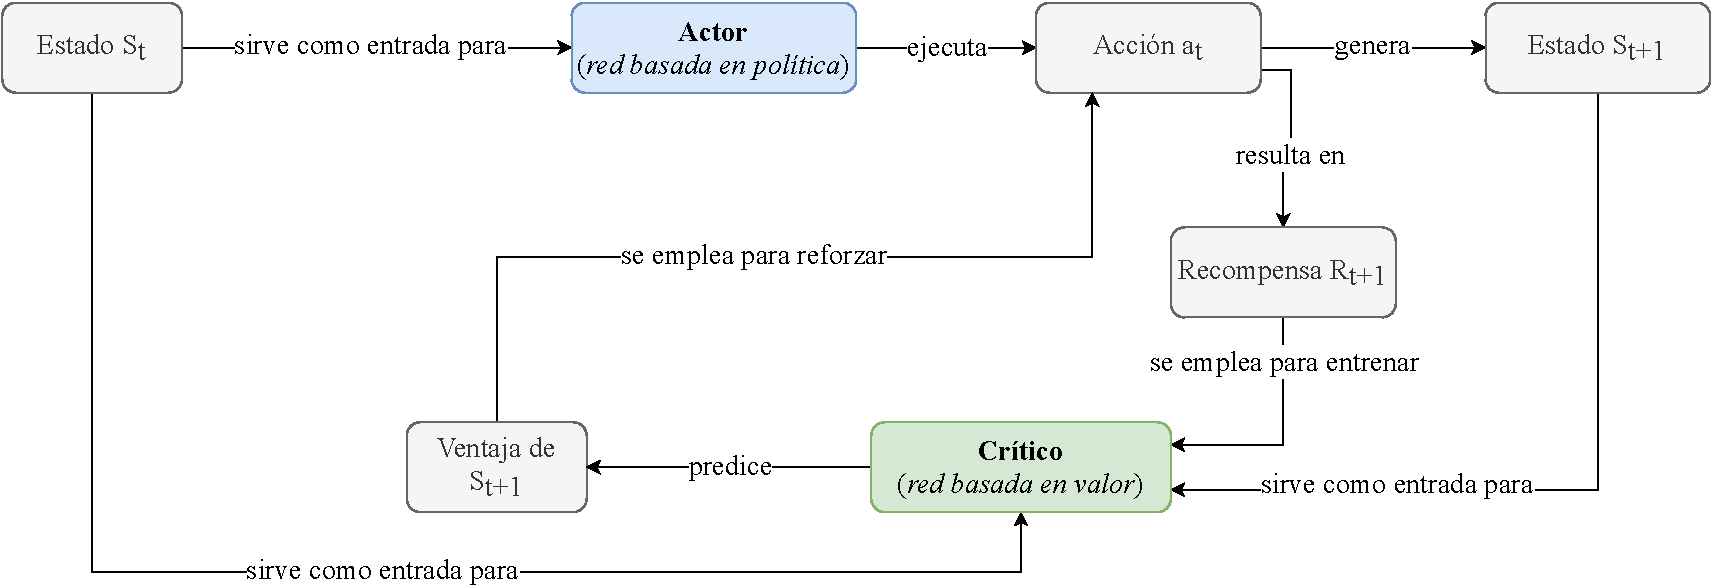
\includegraphics[width=\textwidth]{imagenes/actor-critic.pdf}
    \caption{Funcionamiento de modelos \textit{actor-critic}. Adaptado de \cite{zai2020deep}}
    \label{fig:actor-critic}
\end{figure}

A2C es una versión síncrona de \textbf{A3C} (\textit{Asynchronous Advantage Actor Critic}) \cite{mnih2016asynchronous}. Ambos están basados en la interacción entre diferentes nodos (\textit{\textbf{workers}}) encargados de generar experiencias a partir de una copia propia de la función de valor, la política y el entorno, tal y como se muestra en la Figura \ref{fig:a3c}. Así, en el caso de A3C, tras la recolección de un lote (\textit{batch}) de experiencias, cada \textit{worker} actualiza un \textbf{modelo global} de forma asíncrona, sin existir coordinación alguna con el resto de nodos. Posteriormente, los \textit{workers} actualizan su copia de los modelos y continúan el proceso de aprendizaje.

\begin{figure}
    \centering
    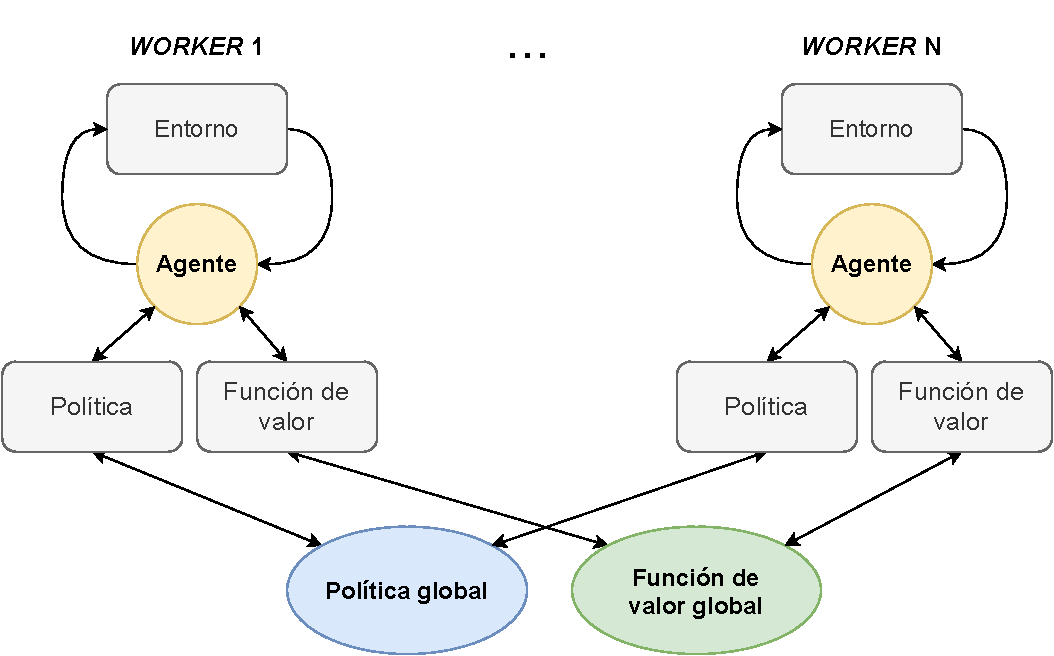
\includegraphics[width=\textwidth]{imagenes/A3C.pdf}
    \caption{Modelo A3C. Adaptado de \cite{morales2020grokking}}
    \label{fig:a3c}
\end{figure}

Por el contrario, A2C es una versión síncrona de A3C que cuenta con un único agente coordinando la interacción con el entorno, tal y como se muestra en la Figura \ref{fig:a2c}. De esta forma, en vez de tener múltiples nodos que actúan y aprenden, pasamos a contar con un único nodo aprendiendo a partir de la experiencia de diferentes actores.

\begin{figure}
    \centering
    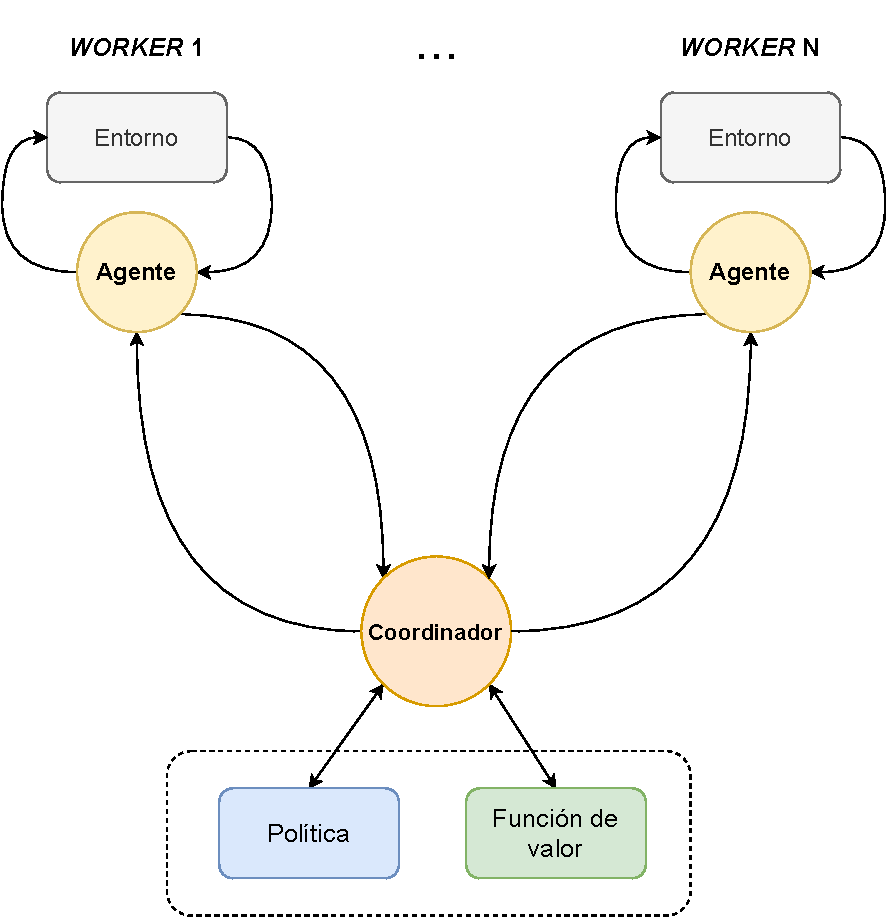
\includegraphics[width=0.7\textwidth]{imagenes/A2C.pdf}
    \caption{Modelo A2C}
    \label{fig:a2c}
\end{figure}

Así, en A2C el nodo \textbf{coordinador} espera a que todos los \textit{workers} terminen su trabajo antes de actualizar los parámetros globales. De esta forma, se consigue que en la siguiente iteración todos los \textit{workers} partan de la misma política. La actualización sincronizada del gradiente permite un entrenamiento más cohesionado, evitando que haya agentes empleando diferentes versiones de la política y logrando que la convergencia sea más rápida con respecto a A3C\footnote{Se ha demostrado que A2C es capaz de hacer un uso más eficiente de las GPUs, así como trabajar mejor con \textit{batches} de gran tamaño. De esta forma, A2C consigue un rendimiento igual o superior al de A3C (\url{https://openai.com/blog/baselines-acktr-a2c/).}}.

Finalmente, al tratarse de un método \textit{on-policy}, se sigue un proceso de aprendizaje similar al de PPO. Además, la función de ventaja previamente definida en la ecuación \ref{advantage} vuelve a ser un factor clave para computar el error y actualizar los pesos. Esta puede aproximarse mediante Monte Carlo (\ref{AdvMC}), empleando el ya conocido $TD$-$error$ ($R_{t+1} + \gamma V(S_{t+1}) - V(S_t)$) (\ref{AdvTD}) o a partir de una estimación \textit{n-step} (\ref{AdvNstep}):

\begin{align}
    A_\varphi(s_t,a_t) \approx\ & R(s_t, a_t) - V_\varphi(s_t) \label{AdvMC} \\
                       \approx\ & r(s_t,a_t,s_{t+1}) + \gamma V_\varphi(s_{t+1}) - V_\varphi(s_t) \label{AdvTD} \\
                       \approx\ & \sum_{k=0}^{n-1}\gamma^k r_{t+k+1} + \gamma^n V_\varphi(s_{t+n+1}) - V_\varphi(s_t) \label{AdvNstep}
\end{align}

A partir de esta función de ventaja, se lleva cabo la actualización de la red \textit{actor} tal que:

\begin{equation}
    \nabla_\theta J(\theta) = \sum_t \nabla_\theta\ log\ \pi_\theta(s_t,a_t) A_\varphi(s_t,a_t)
\end{equation}

Finalmente, el \textit{crítico} se actualiza tratando de minimizar el error $TD$ entre el valor estimado de un estado y su valor real:

    \begin{equation}
            \mathcal{L}(\varphi) = \sum_t A_\varphi(s_t,a_t)^2
    \end{equation}

\subsubsection{DDPG}

\textbf{\textit{Deep Deterministic Policy Gradient}} (\textbf{DDPG}) \cite{lillicrap2015continuous} es un algoritmo \textit{off-policy} de tipo \textit{actor-critic} basado en la combinación de \textbf{DPG} (\textit{Deterministic Policy Gradient}) \cite{silver2014deterministic} con \textbf{DQN}. Puede verse como una versión de DQN adaptada a entornos continuos \cite{zai2020deep}.

Hasta el momento hemos visto agentes que, al seguir una política estocástica $\pi_\theta(s)$, asignan cierta probabilidad a cada una de las acciones disponibles desde un estado $s$. Esto garantiza la exploración en ciertas ocasiones, ya que raramente una acción tendrá una probabilidad nula de ser seleccionada. Así, los métodos basados en valor como DQN tienen como fin converger en una política determinista que actúe de forma voraz tal que: $a_t^* = \underset{a}{argmax}\ Q_\theta(s_t,a)$. La exploración, como ya hemos mencionado, se asegura por medio de una política de comportamiento estocástico, como $\epsilon$-$greedy$, dando lugar a un aprendizaje \textit{off-policy}. 

DDPG, por el contrario, tiene como objetivo entrenar una \textbf{política determinista} parametrizada $\mu_\theta(s)$. Atendiendo al teorema del gradiente de la política \cite{sutton1999policy} tenemos:

\begin{equation}
    J(\theta) = \mathds{E}_{s\sim \rho_\mu}[R(s, \mu_\theta(s))]
\end{equation}

Así, en vez de tratar de maximizar el valor de la función $Q$ en el siguiente estado para obtener la acción voraz correspondiente (como ocurre en DQN), DDPG trata de aproximar la mejor acción en el siguiente estado utilizando una función de política $\mu$ \cite{morales2020grokking}. Por tanto, en comparación con la función de pérdida de DQN:

\begin{align}
    \mathcal{L}_i(\theta_i) = & \mathds{E}_{(s,a,r,s')\sim \mathcal{U}(\mathcal{D})} [(r+\gamma \underset{a'}{max}\ Q(s',a';\theta^-) - Q(s,a;\theta_i))^2] \\
    = & \mathds{E}_{(s,a,r,s')\sim \mathcal{U}(\mathcal{D})}[(r+\gamma Q(s', \underset{a'}{argmax}\ Q(s',a';\theta^-);\theta^-) - Q(s,a;\theta_i))^2]
\end{align}

la ecuación empleada por DDPG para computar el valor de pérdida es la siguiente:

\begin{equation}
    \mathcal{L}_i(\theta_i) = \mathds{E}_{(s,a,r,s')\sim \mathcal{U}(\mathcal{D})}[(r+\gamma Q(s', \mu(s';\phi^-);\theta^-) - Q(s,a;\theta_i))^2]
\end{equation}

En esta expresión podemos ver cómo $\mu$ aprende las acciones voraces determinísticas, a la vez que $\phi$ actúa como red objetivo. Podemos, por tanto, expresar la función objetivo de DDPG como:

\begin{equation}
    J_i(\phi_i) = \mathds{E}_{s\sim \mathcal{U}(\mathcal{D})}[Q(s,\mu(s;\phi);\theta]
\end{equation}

Una vez contamos con un método para entrenar políticas voraces deterministas, el problema que surge es cómo garantizar la exploración en el entrenamiento, ya que si la política no está entrenada, las acciones estrictamente voraces no son suficientes para obtener un comportamiento óptimo. 

Como tantas veces hemos mencionado, es necesario equilibrar exploración con explotación; sin embargo, DDPG aprende una política determinista, por lo que no explorará de forma \textit{on-policy}. Para dar solución a este problema, DDPG añade \textbf{ruido} (gaussiano) a las acciones seleccionadas por la política:

\begin{equation}
    \mu'(s) = \mu_\theta(s) + \mathcal{N}
\end{equation}

De esta forma, DDPG es capaz de extender DQN a entornos continuos siguiendo un enfoque \textit{actor-critic} y aprendiendo una política determinista óptima.

\subsubsection{SAC}

El último algoritmo de DRL empleado en este proyecto es \textbf{\textit{Soft Actor Critic}} (\textbf{SAC}) \cite{haarnoja2018soft}. Se trata de un método \textit{off-policy} de tipo \textit{actor-critic} que permite optimizar una política estocástica (a diferencia de DDPG) en entornos continuos.

Los métodos \textit{on-policy} como PPO o A3C son ineficientes en su aprendizaje debido a que necesitan información completamente nueva después de cada actualización de la política. Una alternativa más eficiente son los métodos \textit{off-policy} basados en Q-learning, como DDPG. Estos cuentan con un mejor rendimiento en el aprendizaje, ya que pueden aprender de forma eficiente a partir de información pasada almacenada en memoria (\textit{experience replay buffer}). Sin embargo, un inconveniente de este tipo de métodos es que son muy sensibles a los hiperparámetros de los que dependen, lo que dificulta su convergencia. SAC orienta sus esfuerzos en facilitar dicha convergencia.

Una característica fundamental de SAC es la \textbf{regularización de la entropía}. La política se entrena para maximizar un equilibrio entre la recompensa esperada y la entropía, la cual actúa como medida de aleatoriedad en el comportamiento del agente. Esto está estrechamente relacionado con el equilibrio entre exploración y explotación: aumentar la entropía da lugar a una mayor exploración, lo que puede acelerar el aprendizaje a largo plazo. También puede evitar que la política converja prematuramente en un óptimo local. 

Así, SAC supera el problema de la convergencia alentando a la política a explorar, evitando asignar una probabilidad muy alta a cualquier acción específica de las posibles. Si añadimos la mencionada entropía a la función objetivo del algoritmo, tenemos:

\begin{equation}
    J(\theta) = \sum_{t=1}^{T} \mathds{E}_{(s_t,a_t) \sim \rho_{\pi_\theta}}[r(s_t,a_t) + \alpha \mathcal{H}(\pi_\theta(\cdot|s_t))]
\end{equation}

donde $\mathcal{H}$ es la medida de entropía y $\alpha$ es un coeficiente que controla la importancia que se otorga a dicha medida\footnote{Este coeficiente $\alpha$ se denomina \textit{temperatura}. Su ajuste no es una tarea trivial, lo que ha llevado al desarrollo de nuevas versiones de SAC orientadas ajustar automáticamente su valor \cite{haarnoja2018soft}.}.

SAC hace uso de tres redes para realizar esta tarea de optimización\footnote{Ecuaciones extraídas de: \url{https://julien-vitay.net/deeprl/}.}:

\begin{enumerate}
    \item Una primera red encargada de aproximar la función de valor $V_\varphi$ (\textit{soft state-value function}) con la siguiente función de pérdida y actualización:
    
        \begin{equation}
            \mathcal{L}(\varphi) = \mathds{E}_{s_t \in \mathcal{D}} [\mathds{E}_{a_{t} \in \pi} [(Q_\psi(s_{t}, a_{t}) - \log \, \pi_\theta(s_t, a_t)] - V_\varphi(s_t) )^2]
        \end{equation}
    
        \begin{equation}
            \nabla_\varphi \mathcal{L}(\varphi) = \nabla_\varphi V_\varphi(s_t) \, (V_\varphi(s_t) - Q_\psi(s_{t}, a) + \log \, \pi_\theta(s_t, a) )
        \end{equation}
    
    \item Otra red encargada de estimar el valor de la función $Q_\psi$ (\textit{soft Q-value function}). Sus funciones de pérdida y actualización son:
    
        \begin{equation}
            \mathcal{L}(\psi) = \mathds{E}_{s_t, a_t \in \mathcal{D}} [(r_{t+1} + \gamma \, V_\varphi(s_{t+1}) - Q_\psi(s_t, a_t))^2]
        \end{equation}
        
        \begin{equation}
            \nabla_\psi \mathcal{L}(\psi) = - \nabla_\psi Q_\psi(s_t, a_t) \, (r_{t+1} + \gamma \, V_\varphi(s_{t+1}) - Q_\psi(s_t, a_t))
        \end{equation}
    
    \item Una última red destinada a aproximar la política estocástica $\pi_\theta$. Esta es entrenada de acuerdo a una función de pérdida que minimiza la divergencia de Kullback-Leibler (KL) \cite{haarnoja2018soft} entre la política actual $\pi_\theta$ y la función \textit{softmax} aplicada sobre los \textit{soft Q-values}:
    
        \begin{equation}
            \mathcal{L}(\theta) = \mathds{E}_{s_t \in \mathcal{D}} [D_\text{KL}(\pi_\theta(s, \cdot) | \frac{\exp Q_\psi(s_t, \cdot)}{Z(s_t)})] 
        \end{equation}
        
        \begin{equation}
            \nabla_\theta \mathcal{L}(\theta) = \nabla_\theta D_\text{KL}(\pi_\theta(s, \cdot) | \frac{\exp Q_\psi(s_t, \cdot)}{Z(s_t)})
        \end{equation}

\end{enumerate}

Finalmente, SAC fue probado y comparado junto a DDPG, PPO y TD3, entre otros algoritmos que constituyen el estado del arte, logrando superarlos en rendimiento y resultados. Por lo general, la ventaja que supone la exploración gracias a la medida de entropía permite que el agente descubra mejores políticas que sus competidores.

\section{Aplicación de DRL en control HVAC}

En los últimos años, el uso de RL y DRL en el control de sistemas de calefacción, ventilación y aire acondicionado (HVAC) ha vivido un crecimiento más que considerable. Con una simple búsqueda en Scopus empleando la cadena de búsqueda ``\texttt{reinforcement} \texttt{learning}'' \texttt{AND} ``\texttt{HVAC}'' podemos apreciar el creciente interés en este campo, pasando de 3 publicaciones en el período 1997--2011 a un total de 37 publicaciones en solamente el año 2020 (ver Figura \ref{fig:scopus}).

\begin{figure}
    \centering
    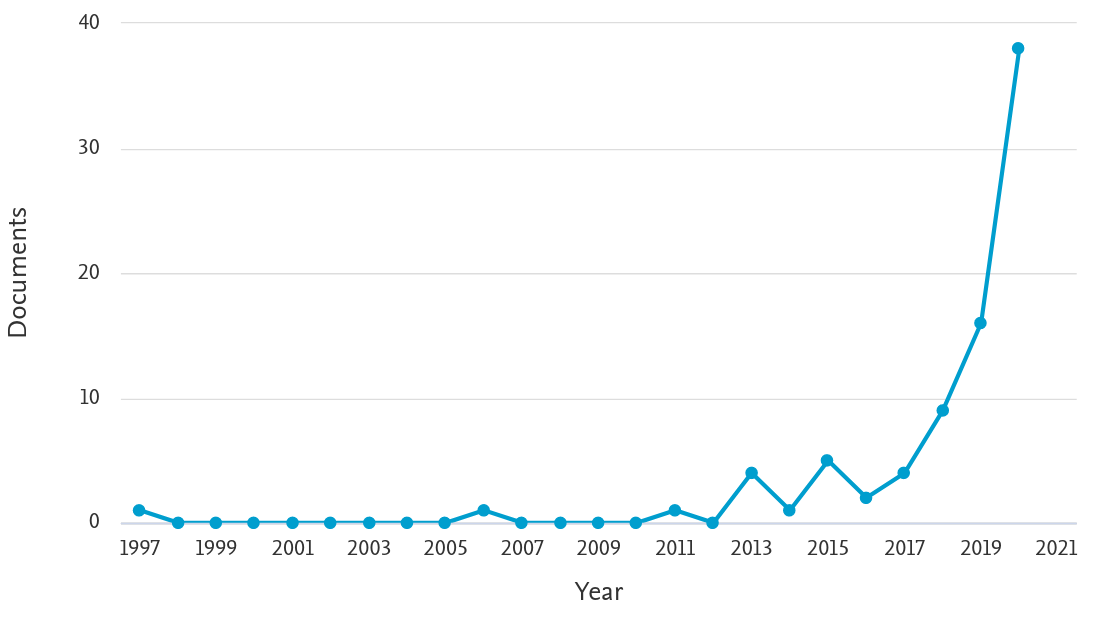
\includegraphics[width=\textwidth]{imagenes/scopus.png}
    \caption{Número de publicaciones relacionadas con aprendizaje por refuerzo y control HVAC en período 1997-2021}
    \label{fig:scopus}
\end{figure}

Este crecimiento se ha visto favorecido por los recientes avances en el campo del aprendizaje por refuerzo, y es que en los últimos años se ha demostrado la factibilidad del control HVAC mediante DRL empleando espacios de acciones reducidos y modelos de edificios simplificados \cite{zhang2019whole, vazquez2019fusing, moriyama2018reinforcement}.

La mayoría de las propuestas en la literatura destinadas a control HVAC mediante DRL hacen uso de diferentes herramientas de simulación energética de edificios, tales como EnergyPlus \cite{wetter2019ibpsa} o Modelica \cite{bucsoniu2018reinforcement}, facilitando así el entrenamiento y la experimentación. El uso de este tipo de simuladores se debe a que el entrenamiento de un agente de DRL en un escenario real sería demasiado ineficiente, debido a la necesidad de establecer un mapeo completo entre estados, acciones y recompensas considerando casos extremos \cite{brandi2020deep}. Además, se requiere de un entrenamiento de entre 20 y 50 días para converger en una política de control aceptable \cite{fazenda2014using, costanzo2016experimental, vazquez2019fusing}, lo que dificulta aún más el entrenamiento directo de algoritmos de DRL en entornos reales. Normalmente, los simuladores suelen combinarse con librerías de \textit{deep learning} (ej. TensorFlow/Keras, Pytorch) o DRL directamente (ej. Stable Baselines, RLlib) para pre-entrenar y probar los algoritmos en los entornos simulados antes de su despliegue \cite{wang2017long, valladares2019energy}.

\subsection{Formulación del problema}
\label{sec:formulacion}

Uno de los principales motivos que empujan al uso de DRL en control HVAC es la búsqueda de \textbf{ahorro energético}. De hecho, los sistemas basados en DRL han logrado conseguir una mayor eficiencia en comparación con los controladores tradicionales basados en reglas \cite{brandi2020deep, zhang2019whole, zhang2018deep, vazquez2019fusing, vazquez2017balancing}.

Por otro lado, los algoritmos de DRL destinados a control HVAC no tienen como único fin reducir el consumo energético, sino también garantizar una serie de requisitos de temperatura o \textbf{confort}\footnote{Es importante destacar que la definición de los estados o recompensas puede contemplar otras variables más allá de la temperatura tales como, por ejemplo, la concentración de CO$_2$ en el aire o la humedad.} \cite{wei2017deep, fazenda2014using, dalamagkidis2007reinforcement}.

Existen diferentes formas de medir el confort, tales como:

 \begin{itemize}
    \item La distancia entre la temperatura actual y la deseada: 
    
        \begin{equation}
            f(T, \hat{T}) = |T - \hat{T}|
        \end{equation}
        
    \item La distancia al cuadrado:
    
        \begin{equation}
            f(T, \hat{T}) = (T - \hat{T})^2
        \end{equation}
    
    \item La distancia a un rango de \textit{confort} objetivo:
    
        \begin{equation}
            f(T, T_{lower}, T_{upper}) = |T - T_{inf}|_+ + |T - T_{sup}|
        \end{equation}
    
    \item La distancia a la temperatura objetivo y al rango de confort según el estándar 55 de ASHRAE \cite{ansi2004standard}, el cual define un rango de temperatura aceptable de entre 23--26ºC para verano y 20--23.5ºC para invierno. Esto es:
    
        \begin{equation}
            f(T, \hat{T}, T_{inf}, T_{sup}) = |T - \hat{T}|_+ + (T - T_{sup})_+^2 + (T - T_{inf})^2
        \end{equation}
    
    \item Funciones no lineales como \textit{softplus}, gaussiana truncada, etc.
\end{itemize}

Mientras que algunos autores consideran que el confort de los ocupantes de un edificio es una restricción a la que siempre hay que dar prioridad, otros se centran en lograr un equilibrio entre dicho confort y el consumo de energético \cite{vazquez2019reinforcement}. 

Por tanto, el objetivo perseguido en el control HVAC de edificios no es otro que el de encontrar la política óptima que maximice el confort y minimice el consumo energético al mismo tiempo. Concretamente, buscamos una política, $\pi$, que implique la mayor cantidad de estados deseables posible y la menor cantidad de acciones energéticamente costosas.

Así, partiendo de un conjunto de \textbf{estados} u observaciones definidos por las condiciones ambientales del entorno, se plantean los siguientes objetivos:

\begin{itemize}
    
    \item Con respecto al consumo energético (medido en \textit{kWh}), buscamos la política que conduzca a su minimización, esto es:
        \begin{equation}
            \pi^* = \underset{\pi_\theta}{argmin}\sum^T_{t=1}\ coste(A_t)
        \end{equation}

    \item En el caso del confort, buscamos minimizar la diferencia entre el estado actual del edificio y el objetivo. Podemos definirlo tal que:
        \begin{equation}
            \pi^* = \underset{\pi_\theta}{argmin}\sum^T_{t=1}\ f(S_t, S_{objetivo})
        \end{equation}
    
    Un estado será deseable si las variables o condiciones ambientales que lo componen se encuentran dentro de las preferencias del usuario. Decimos que se produce una \textit{violación del confort} si la temperatura en el estado actual se encuentra fuera de los límites definidos por el usuario.
    
\end{itemize}

Vistos los objetivos a perseguir, podemos combinar la minimización del consumo energético y la maximización del confort en una sola expresión:

\begin{equation}
    \pi^* = \underset{\pi_\theta}{argmin}\sum^T_{t=1} w_t \cdot f(S_t,S_{objetivo}) + (1 - w_t) \cdot coste(A_t)
\end{equation}

siendo $w_t$ y $(1 - w_t)$ los pesos asignados a confort y consumo\footnote{Como puede observarse, $w$ puede ser variable en el tiempo ($w_t$) o incluso depender de otras variables como, por ejemplo, el número de ocupantes del edificio.}, respectivamente. Sobre esta base, podemos definir nuestra función de \textbf{recompensa} tal que:

\begin{equation}
    \label{eq:reward}
    r(S_t,A_t) = (1-w_t) \cdot \lambda_e \cdot coste(A_t) + w_t \cdot \lambda_c \cdot f(S_t,S_{objetivo})
\end{equation}

donde $coste(A_t)$ es el consumo energético; $f(S_t, S_{objetivo})$ es la función que mide el confort; $w$ y $(1-w)$ son los pesos asignados a cada parte de la recompensa, y $-\lambda_e$ (medido en $1/W$) y $-\lambda_c$ (medido en $1/\text{º}C$), sendos factores de escala empleados para eliminar las dimensiones del consumo y la temperatura\footnote{Es común definir dicha función de recompensa en términos negativos con el fin de que el objetivo sea maximizarla (aproximarla a $0$). Esto es: $r(S_t,A_t) = - (1-w_t) \cdot \lambda_e \cdot coste(A_t) - w_t \cdot \lambda_c \cdot f(S_t,S_{objetivo})$. Se trata de la función de recompensa estándar empleada internamente por Energym.}.

Finalmente, las \textbf{acciones} a realizar sobre el entorno y que darán lugar a una determinada recompensa dependerán del problema al que nos encontremos. En el problema tratado en este trabajo, las acciones consistirán en ajustar los \textit{setpoints} de calefacción y refrigeración, tal y como es habitual en control HVAC \cite{vazquez2017balancing, wei2017deep, fazenda2014using}. Un \textit{setpoint} marca la temperatura límite a partir de la cual deberá activarse un sistema de calefacción o refrigeración. En caso de fijar un \textit{setpoint} para calor y otro para frío, el objetivo será mantener el edificio dentro del intervalo entre ambos valores. Cabe destacar que, dependiendo del tipo de problema, el espacio de acciones podrá ser:

\begin{itemize}
    \item \textbf{Discreto}: existe un número finito de acciones donde cada acción es una tupla con valores de \textit{setpoints} fijos.
    \item \textbf{Continuo}: cada \textit{setpoint} es un número real a ajustar.
\end{itemize}

Finalmente, no todos los problemas de control HVAC residen en el ajuste de \textit{setpoints}: otras posibles acciones podrían consistir en regular la potencia de ventilación, o la apertura y cierre de ventanas \cite{chen2018optimal}, entre muchas otras. 

En conclusión, todo problema de control HVAC destinado a ser resuelto mediante RL cuenta con los siguientes componentes:

\begin{itemize}
    \item Una serie de \textbf{estados} u observaciones compuestos por las condiciones ambientales del entorno: temperatura externa/interna, humedad, luminosidad, concentración de CO$_2$, etc., en un momento dado.
    \item Una función de \textbf{recompensa} donde se combinan de forma ponderada el consumo energético (a minimizar) y el confort (a maximizar).
    \item Un espacio de \textbf{acciones} consistentes, en este caso, en la regulación de los \textit{setpoints} para calefacción y refrigeración. Dicho espacio de acciones puede ser discreto o continuo.
\end{itemize}

\subsection{Estado del arte}
\label{sec:estado-del-arte}

Una vez introducido el uso de DRL en control HVAC, pasamos a revisar algunas de las aportaciones más novedosas de la literatura científica en los últimos años.

En el año 1997 tenemos la primera aproximación al uso de RL en control HVAC de la mano de Anderson et al. \cite{anderson1997synthesis}. En este trabajo, se propuso el uso de RL en combinación con control proporcional-integral (PI) para el control de una bobina de calor (\textit{heating coil}). Un año más tarde, en 1998, tuvo lugar la primera aplicación directa de RL en control HVAC, \cite{mozer1998neural}, donde Mozer expuso su \textit{Neural Network House} basada en el control automático de agua caliente, HVAC e iluminación, buscando así reducir el consumo energético y garantizar el bienestar de sus ocupantes.

Desde ese momento, se han ido desarrollando una gran cantidad de trabajos centrados en la reducción del gasto energético de edificios y su gestión inteligente. Algunos ejemplos son: \cite{sun2015event}, donde se consiguió minimizar el consumo energético en un entorno con múltiples estancias; \cite{liu2006experimental,liu2007evaluation}, donde se proponen métodos híbridos orientados a gestionar sistemas de agua fría en grandes centros comerciales, o \cite{costanzo2016experimental}, centrado en la reducción del consumo energético en sistemas de aire acondicionado.

Un factor importante a considerar en la regulación de \textit{setpoints} para calefacción y refrigeración es la ocupación de los edificios. Este factor fue considerado por Barrett \& Linder en \cite{barrett2015autonomous}, donde consiguieron reducir en un 10\% los costes energéticos derivados de dispositivos HVAC empleando RL. De forma similar, en el caso de \cite{urieli2013learning, ruelens2015learning}, se investigaron métodos basados en \textit{set-back} orientados a relajar los requisitos de temperatura cuando no hay personas en el edificio.

Otros ejemplos de aplicaciones de RL destinadas a incrementar la conservación de energía en edificios son \cite{li2015multi, vazquez2017balancing, vazquez2019fusing, dalamagkidis2007reinforcement, yu2010online, yuan2020study, azuatalam2020reinforcement} donde tanto el ahorro energético como el confort fueron tenidos en cuenta para optimizar el funcionamiento de dispositivos HVAC en diferentes entornos. En \cite{brandi2020deep}, se logró un ahorro de entre un 5\% y un 12\% en el control del sistema de calefacción de un edificio de oficinas haciendo uso de un agente basado en \textit{Double DQN}. Por otro lado, Zhang et al. \cite{zhang2019whole, zhang2018deep} lograron reducir en un 16.7\% la demanda energética en un edificio de oficinas empleando A3C, mientras que Vázquez-Canteli et al. \cite{vazquez2019fusing, vazquez2017balancing} lograron un 10\% de ahorro energético aplicando DQN en el control de una bomba de calor. Destaca el caso de Dalamagkidis et al. \cite{dalamagkidis2007reinforcement}, donde los niveles de CO$_2$ también se tuvieron en cuenta como métrica de confort.

Un trabajo reciente y de especial interés es el de Azuatalam et al. \cite{azuatalam2020reinforcement}, donde se llevó a cabo una completa revisión del estado del arte en control HVAC mediante RL, proponiendo una arquitectura capaz de alcanzar un 22\% de ahorro energético semanal.

Finalmente, en \cite{du2008two}, se propone un modelo \textit{actor-critic} orientado a reducir el error en el ajuste de \textit{setpoints} de sistemas HVAC, mientras que en \cite{henze2003evaluation} se llevó a cabo una investigación orientada a probar la eficacia del RL en sistemas de almacenamiento de frío en edificios comerciales.

Como puede verse, contamos con una importante base teórica y práctica sobre la cual se fundamenta el control HVAC por medio de RL y DRL. En esta sección se ha tratado de reflejar parte de la literatura existente, mostrando el amplio abanico de posibilidades que este campo ofrece, y abriendo la puerta al lector a consultar recientes revisiones de la literatura como \cite{vazquez2019reinforcement, mason2019review} en caso de buscar una mayor profundización.

Ya mencionamos en el Capítulo \ref{ch:1} que la mayor parte de los sistemas de control HVAC basados en RL y DRL presentes en la literatura son difícilmente reproducibles y comparables \cite{vazquez2019reinforcement}. No existe, hasta el momento, ningún \textit{framework} (más allá de los brevemente propuestos en \cite{vazquez2019reinforcement}, \cite{azuatalam2020reinforcement}) o \textit{benchmark} destinados a constituir un marco común desde el que comparar modelos de RL y DRL en diferentes climas y entornos. Así, tomando como referencia la arquitectura basada en OpenAI Gym y EnergyPlus propuesta por Zhang et al. en \cite{zhang2018practical, zhang2019whole}, el objetivo de este trabajo será proponer una solución a este problema, tratando de desarrollar un ecosistema de simulación común que pueda ser empleado para validar cualquier nueva aportación al campo.


